\documentclass [9pt] {beamer}

\usepackage{color}
\usepackage{beamerthemeshadow, amsmath, amssymb}
\usepackage{subfigure}
\usepackage{amsfonts}
\usepackage{graphics}
\usepackage{graphicx}
\usepackage{epsfig}
\usepackage{textcomp}
\usepackage[english]{babel}
\usepackage{verbatim}
%\usepackage[latin1]{inputenc}
\setbeamercolor{footnote}{fg=blue}
%\usecolortheme{crane}
\usetheme{Copenhagen}
%\usetheme{Warsaw}
\beamertemplatesolidbackgroundcolor{white!25}
\setlength{\parskip}{8pt plus .5pt minus .5pt}
\setbeamertemplate{footline}[frame number]
\logo{\includegraphics[height=1.2cm]{logo}}


\title[JIITN]{\LaTeX: The Language of Scientific Writing}
\subtitle{TEQIP-III Sponsored FDP}
\institute[]{
\textbf{\small Presented By :}\\
\small Dr. Mukesh Saraswat \\saraswatmukesh@gmail.com\\ Raju Pal\\ raju3131.pal@gmail.com\\[1.5cm]
\begin{center}
\textbf{\small Jaypee Institute of Information Technology, Noida}
\end{center}

}

\date{11-15 June, 2018}

\begin{document}
\frame[plain]{\titlepage}

%\begin{frame}[shrink]%[allowframebreaks]%
%\frametitle{Outline}
%%\transboxout
%\transdissolve
%%\tableofcontents{}
%\tableofcontents[hideallsubsections]
% %[pausesections]
%\end{frame}
%\section*{Outline of the Workshop}
\begin{frame}[plain]{Outline of FDP}
\begin{itemize}
	\item Motivation\\[0.3cm]
	\item Installation of \LaTeX \ software on Windows\\[0.3cm]
	\item Report Writing\\[0.3cm]
	\begin{itemize}
		\item \LaTeX \ commands\\[0.2cm]
		\item JabRef and its utility
	\end{itemize}
	\item Thesis Writing\\[0.3cm]
	\item Paper Writing: IEEE, Elseviers, Springer\\[0.3cm]
	\item Presentation using \LaTeX\\[0.3cm]
	\item Resume/Letter/synopsis 
	
	
\end{itemize}
\end{frame}
\section{Introduction}
%\subsection{Deterministic and  Probabilistic Approach}\label{dpa}
\subsection{Problems in writing Thesis/Paper}\label{Problems in writing Thesis/Paper}

\begin{frame}\frametitle{Problems in writing Thesis/Paper}
\rm
\fontsize{9pt}{11pt}\selectfont
\begin{itemize}
\fontsize{8pt}{10pt}\selectfont
\item Formatting ( Single Column, Two Column) \\[.30cm]

\item Reference Management\\[.30cm]
\item Figure Management\\[.30cm]

\item Table Management\\[.30cm]

\item List of Figures\\[.30cm]

\item List of Tables\\[.30cm]
\item ....Many more
\end{itemize}
\end{frame}


\begin{frame}%\frametitle{Solution is Latex}
\begin{center}
\Huge\textcolor[rgb]{0.98,0.00,0.00}{\textbf{Solution is Latex}}
\end{center}
\end{frame}



\subsection{Latex}\label{Latex}

\begin{frame}\frametitle{Introduction}\transblindshorizontal
\rm
%\fontsize{9pt}{1.1pt}\selectfont
\begin{itemize}
\fontsize{8pt}{10pt}\selectfont
\item Pronounced: \textcolor[rgb]{1.00,0.00,0.00}{``Lay-tech"}. \\[.30cm]

\item Latex ---- universal typesetting tools for academic research community. Math, Physics, Engineering, Finance ...\\[.30cm]
\item Supported by nearly all the publishing corporations: \\\textcolor[rgb]{0.98,0.00,0.00}{IEEE, ACM, Elsevier, Springer, Wiley, etc.}\\[.30cm]

\item Almost all the IEEE Journals are published as a classic Latex Style\\[.30cm]

\item TeX: computer program released in 1982 by \textcolor[rgb]{0.98,0.00,0.00}{Donald E. Knuth}:\\
\textcolor[rgb]{1.00,0.00,0.00}{A revolution in typesetting}\\[.30cm]

\item Later, a mathematician and computer scientist, \textcolor[rgb]{0.98,0.00,0.00}{Leslie Lamport}, wrote a variant of TEX called LaTeX that focuses on
document structure:\\
\textcolor[rgb]{0.98,0.00,0.00}{Packages to make TeX easier to use}\\[.30cm]

\item Low level markup language and case sensitive
\end{itemize}
\end{frame}

\begin{frame}{Softwares for programming or writing the .tex codes}
\begin{itemize}
	\item Windows:\\
	MikTeX, TeXmaker, WinEdt, LyX and so on
	\item Linux like ubuntu:\\
	TeX-Live, Kile, LyX, and so on
	\item Mac OS:\\
	MacTeX, LyX
\end{itemize}
\end{frame}

\begin{frame}{TeX vs. LaTeX}
\begin{itemize}
	\item TeX can recognize only .ps files for images
	\item LaTeX can recognize .jpg files for images
	\item BibTeX is used for Bibliography i.e. giving references
	\item Recently some ways have been discovered to overcome this limitation. 
\end{itemize}
\end{frame}

\begin{frame}\frametitle{Advantages of Latex}
\rm
\fontsize{9pt}{11pt}\selectfont
\begin{itemize}
\fontsize{8pt}{10pt}\selectfont

\item It is efficient for using on publication of books or articles.\\[.30cm]

\item It can save  user's time by automatically formatting the sections, equations, and pictures of the documents.\\[.30cm]

\item Users need only to learn a few simple commands, which specify the logical structure of a document.\\[.30cm]

\item Complex structures such as footnotes, references, table of contents, and bibliographies can be generated easily.\\[.30cm]

\item \textcolor[rgb]{0.98,0.00,0.00}{LaTeX is highly portable and free}
\end{itemize}
\end{frame}

\begin{frame}\frametitle{Advantages of Latex}
\rm
\fontsize{9pt}{11pt}\selectfont
\begin{itemize}
\fontsize{8pt}{10pt}\selectfont
\item High typeset quality\\[.30cm]

\item Easy to include math formulas\\[.30cm]

\item Source file format is not bounded to a particular OS or platform\\[.30cm]

\item Latex implementations exists for all platforms (DOS, Windows, Linux,..)\\[.30cm]

\item Good for large documents\\[.30cm]

\end{itemize}
\end{frame}
%
%
\begin{frame}\frametitle{Advantages of Latex}
\rm
\begin{figure}[h!]
\begin{center}
    %\centering
     \includegraphics[width=0.6\textwidth]{Picture1.eps}
\end{center}
\end{figure}
\end{frame}


\begin{frame}\frametitle{Disadvantages of Latex}
\rm
\fontsize{9pt}{11pt}\selectfont
\begin{itemize}
\fontsize{8pt}{10pt}\selectfont

\item Maybe hard to use at the beginning.\\[.30cm]

\item Don't support WYSIWYG (``what you see is what you get"):\\
\textcolor[rgb]{0.98,0.00,0.00}{except lyx or next version Tex}\\[.30cm]

%\item Somehow low efficiency to prepare a presentation.\\[.30cm]
\end{itemize}
\end{frame}

\begin{frame}\frametitle{How LaTeX Works}
\rm
\fontsize{9pt}{11pt}\selectfont
\begin{itemize}
\fontsize{8pt}{10pt}\selectfont

\item LaTeX source editor + LaTeX compiler (*.tex).\\[.30cm]

\item Like C + Borland C compiler\\[.30cm]

\item Many LaTeX compilers.\\[.30cm]
\item Popular LaTeX IDE for Windows:
 \textcolor[rgb]{0.98,0.00,0.00}{WinEdit + MiKTeX}\\
  http://www.miktex.org/ + http://www.winedt.com/\\[.30cm]
\item Popular LaTeX IDE for Linux:
\textcolor[rgb]{0.98,0.00,0.00}{Kile + eTeX or encTeX or MiKTeX}\\
http://kile.sourceforge.net/
\end{itemize}

\begin{center}
\Huge\textcolor[rgb]{0.98,0.00,0.00}{\textbf{For Any Problem $\Longrightarrow$ Google}}
\end{center}
\end{frame}

%
%
\begin{frame}{MikTex on Windows}%{Optional Subtitle}
  \begin{itemize}
  \item {Download the MikTex Software.}
  \item Go to link: https://miktex.org/download 
    
  \end{itemize}
\begin{figure}
	\subfigure{
		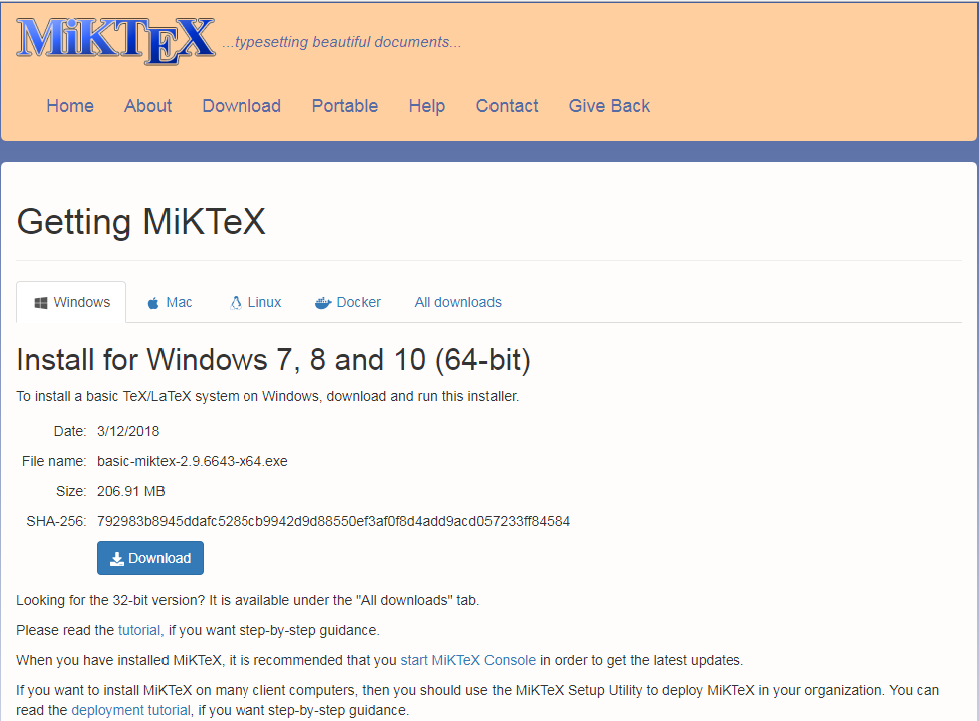
\includegraphics[width=0.8\textwidth,height=0.7\textheight]{fig1.png}}
	%\caption{Step 1: Download the MikTex Software: https://miktex.org/download}
\end{figure}
\end{frame}

\begin{frame}{MikTex on Windows}%{Optional Subtitle}
\begin{itemize}
\item {Step 2: Install the software as per the guided steps.}
\end{itemize}
\end{frame}


\begin{frame}{MikTex on Windows}%{Optional Subtitle}
\begin{figure}
\subfigure[Step 3: Open the MikTex Console and Select the operation mode.]{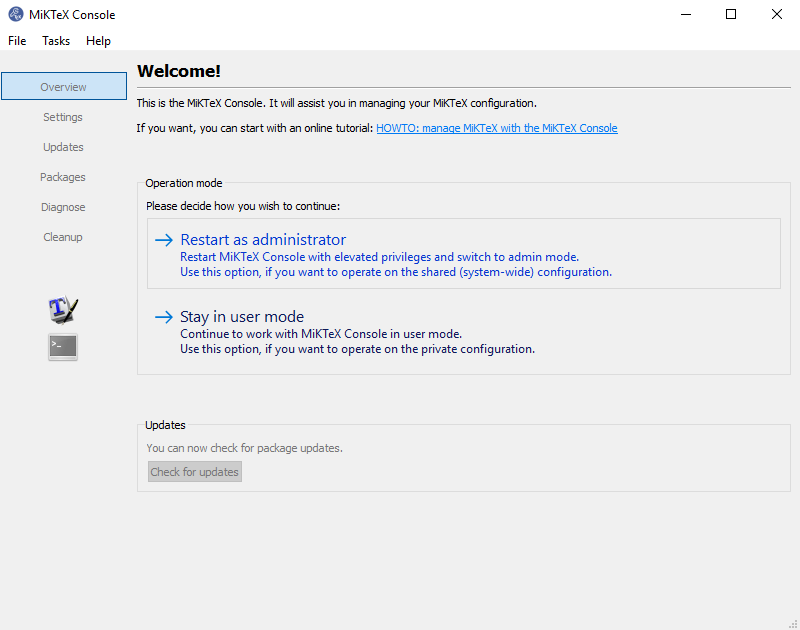
\includegraphics[width=0.7\textwidth,height=0.7\textheight]{fig44.png}}
\end{figure}
\end{frame}

\begin{frame}{MikTex on Windows}%{Optional Subtitle}
\begin{figure}
\subfigure[Step 4: Change the package repository.]{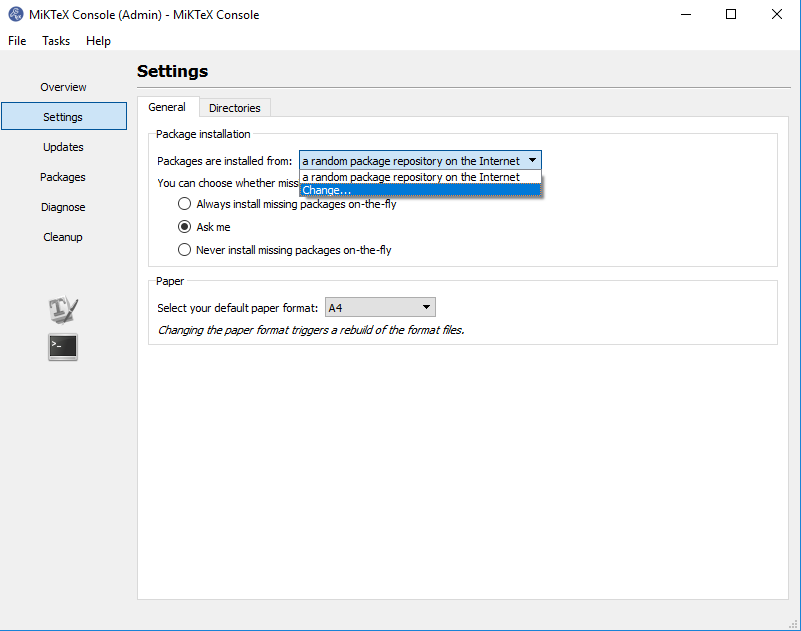
\includegraphics[width=0.7\textwidth,height=0.7\textheight]{fig3.png}}
\end{figure}
\end{frame}

\begin{frame}{MikTex on Windows}%{Optional Subtitle}
\begin{figure}
\subfigure[Step 5: Check the Connection Settings.]{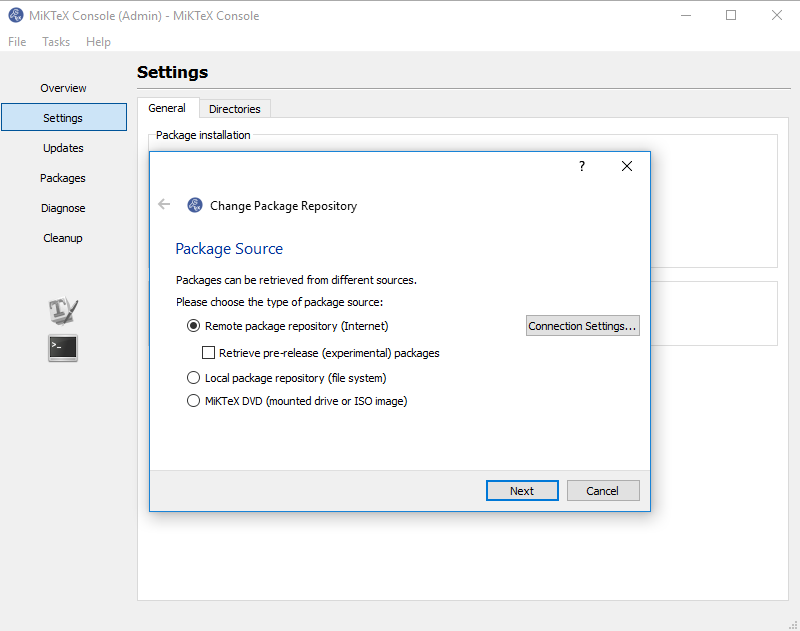
\includegraphics[width=0.7\textwidth,height=0.7\textheight]{fig4.png}}
\end{figure}
\end{frame}

\begin{frame}{MikTex on Windows}%{Optional Subtitle}
\begin{figure}
\subfigure[Step 6: Select the repository.]{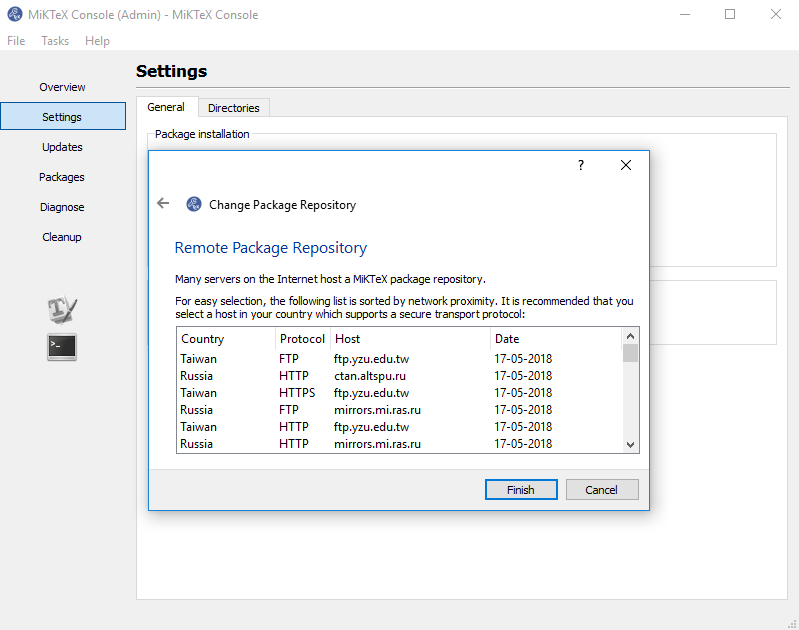
\includegraphics[width=0.7\textwidth,height=0.7\textheight]{fig5.png}}
\end{figure}
\end{frame}

\begin{frame}{MikTex on Windows}%{Optional Subtitle}
\begin{figure}
\subfigure[Step 7: Check package updation.]{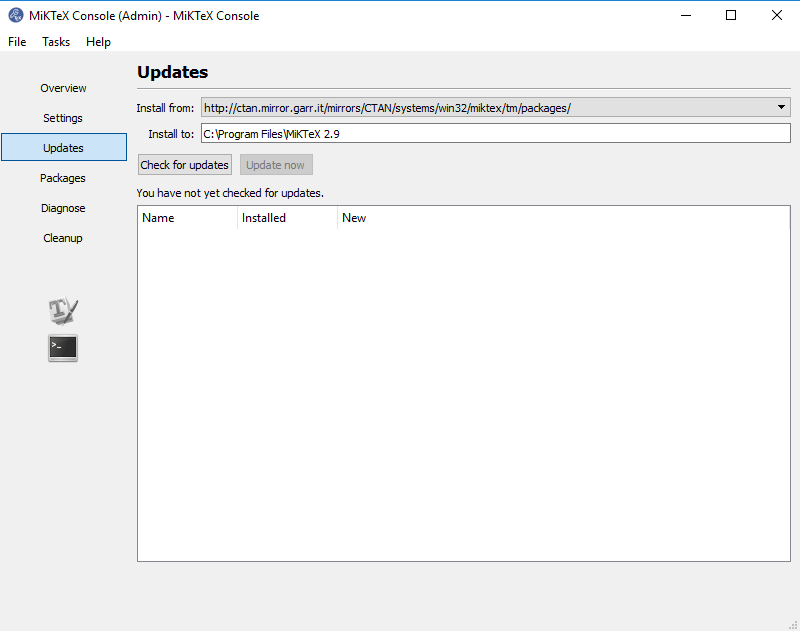
\includegraphics[width=0.7\textwidth,height=0.7\textheight]{fig6.png}}
\end{figure}
\end{frame}

\begin{frame}{MikTex on Windows}%{Optional Subtitle}
\begin{figure}
\subfigure[Step 8: If any, perform package updation.]{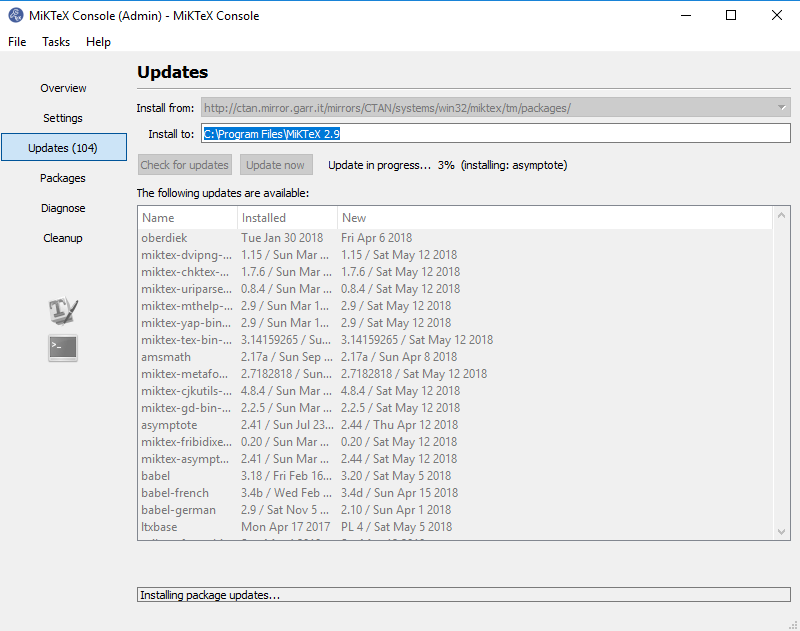
\includegraphics[width=0.7\textwidth,height=0.7\textheight]{fig7.png}}
\end{figure}
\end{frame}















\begin{frame}\frametitle{How LaTeX Works}
\rm
\begin{figure}[h!]
\begin{center}
    %\centering
     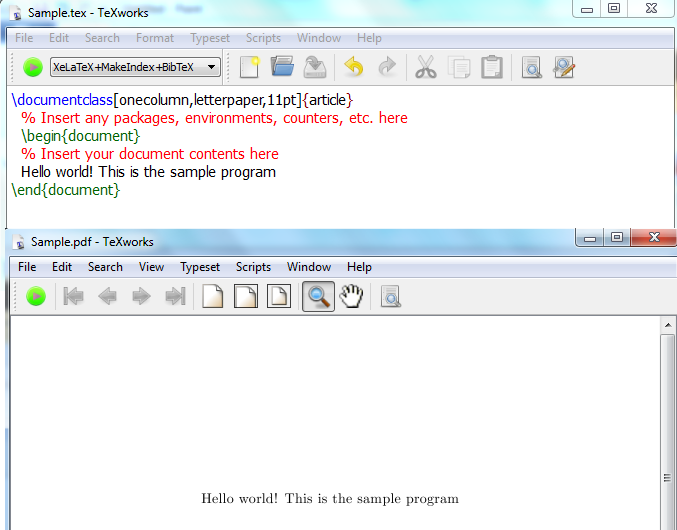
\includegraphics[width=0.8\textwidth]{home} \\
\end{center}
\end{figure}
\end{frame}

%\begin{frame}\frametitle{Important features of using professional editors}
%\rm
%\fontsize{9pt}{11pt}\selectfont
%\begin{itemize}
%\fontsize{8pt}{10pt}\selectfont
%
%\item Highlight keywords\\[.30cm]
%\item Automatic packages download\\[.30cm]
%\item Auto completion\\[.30cm]
%\item Keywords reminders\\[.30cm]
%\item One Key functions\\[.30cm]
%\item Free of memorizing many symbols, keywords, environment names\\[.30cm]
%\end{itemize}
%\end{frame}
%
%\subsection{Common Commands}\label{Common commands}
%\begin{frame}\frametitle{Common commands}
%\rm
%\fontsize{9pt}{11pt}\selectfont
%\begin{itemize}
%\fontsize{8pt}{10pt}\selectfont
%
%\item \textcolor[rgb]{0.98,0.00,0.00}{latex} sample.tex (.. smaple.dvi)\\[.30cm]
%\item \textcolor[rgb]{0.98,0.00,0.00}{dvipdf} sample.dvi (.. sample.pdf)\\[.30cm]
%\item \textcolor[rgb]{0.98,0.00,0.00}{dvips} sample.dvi (.... sample.ps)\\[.30cm]
%\item \textcolor[rgb]{0.98,0.00,0.00}{pdflatex} sample.tex (..sample.pdf)\\[.30cm]
%\item \textcolor[rgb]{0.98,0.00,0.00}{bibtex}...\\[.30cm]
%\end{itemize}
%\end{frame}


\subsection{Required Components of a LaTeX Document}\label{Required Components of a LaTeX Document}
\subsection{Required Components}\label{Required Components}
\begin{frame}\frametitle{Required Components of a LaTeX Document}
\rm
\fontsize{9pt}{11pt}\selectfont
\begin{itemize}
\fontsize{8pt}{10pt}\selectfont

\item Every LaTeX document must contain the following three components. Everything else is optional (even text).\\[.30cm]
\begin{enumerate}
  \item \textcolor[rgb]{0.98,0.00,0.00}{$\backslash$documentclass\{article\}}\\[.30cm]
  \begin{itemize}
    \item Tells LaTeX what kind of document it is to process:article, report, book, etc.\\[.30cm]
    \item The default font size for each class is 10 point.\\[.30cm]
    \item \textcolor[rgb]{0.98,0.00,0.00}{$\backslash$documentclass[11pt]\{article\}} or \textcolor[rgb]{0.98,0.00,0.00}{$\backslash$documentclass[12pt]\{article\}}\\[.30cm]
    \item Required information is included in LaTeX commands in braces \{\}.\\[.30cm]
    \item Optional information is included in square brackets []
  \end{itemize}
  \item \textcolor[rgb]{0.98,0.00,0.00}{$\backslash$begin\{document\}}\\[.30cm]
  \item \textcolor[rgb]{0.98,0.00,0.00}{$\backslash$end\{document\}}\\[.30cm]
\end{enumerate}
\end{itemize}
\end{frame}

\section{Learn by examples}\label{Learn by examples}
\subsection{Example 1. Basic}\label{Example 1. Basic}
\begin{frame}\frametitle{Learn by examples}
\rm
\fontsize{9pt}{11pt}\selectfont

\textbf{Example 1. Basic}\\[.30cm]

$\backslash$documentclass\{article\}\\
$\backslash$begin\{document\}\\
This is my $\backslash$emph\{first\} document prepared in $\backslash$LaTeX.\\
$\backslash$end\{document\}\\[0.5cm]

\textbf{Note:} Select pdfLateX+MakeIndex+BibTeX from the top menu bar and hit F5 or run icon or ctrl+T
\end{frame}

\subsection{Example 2. Play with text}\label{Example 2. Play with text}

\begin{frame}\frametitle{Learn by examples}
\rm
\fontsize{9pt}{11pt}\selectfont

\textbf{Typesetting Text}\\[.30cm]
\begin{itemize}
\item $\backslash$$\backslash$ or $\backslash$newline and $\backslash$newpage
\item For quotes, use {\tt ``} (two backquotes) and {\tt ''} (two
apostrophes) instead of {\tt "}. For single quotes, just use
\texttt{`} and \texttt{'}.
\item Bold  \textbf{$\backslash$textbf\{\dots\}} or \textbf{\{$\backslash$bf \dots\}}
\item Italics \textbf{$\backslash$emph\{\dots\}} or \textbf{$\backslash$textit\{\dots\}} or \textbf{\{$\backslash$it \dots\}}
\item Underline \textbf{$\backslash$underline\{\dots\} }
\item Color \textcolor{orange}{\textbf{$\backslash$textcolor\{name of color\}\{\dots\} }} or {\color{red}\{{\textbf{$\backslash$color\{name of color\}\dots\} }}}. You have to use $<$xcolor$>$ package.
\item The predefined color names are:\\

black, blue, brown, cyan, darkgray, gray, green, lightgray, lime, magenta, olive, orange, pink, purple, red, teal, violet, white, yellow
\item New colors are defined as \{in preamble\}:

\textbf{$\backslash$definecolor\{name\}\{RGB\}\{10,20,30\}}

\end{itemize}
\end{frame}

\begin{frame}\frametitle{Learn by examples}
\rm
\fontsize{9pt}{11pt}\selectfont

\textbf{Exercise 2. Play with text}\\[.30cm]
\begin{itemize}
	\item Write a LaTeX code for the content given in \textbf{Ex2\_1.pdf}
	\item Write a LaTeX code for the content given in \textbf{Ex2\_2.pdf}
	
\end{itemize}

\end{frame}


\begin{frame}\frametitle{Learn by examples}
\rm
\fontsize{9pt}{11pt}\selectfont
\begin{itemize}
  \item Consecutive whitespace characters (blank or tab) are treated as one space.\\[.30cm]
  \item Paragraphs must be separated by at least one line in the .tex file.\\[.30cm]
  \item Comments can be added using the \% character. Any text on a line after \% will be ignored by the \TeX compiler.
  \item Special Characters:
  \begin{itemize}
    \item The following symbols are reserved:\\
            \# \ \  \$ \ \  \% \ \  \& \ \  \_ \ \  \{ \ \  \} \ \  \^{} \ \  \~{} \ \  $\backslash$

    \item To include them in your text:\\
         $\backslash$\# \ \ $\backslash$\$ \ \ $\backslash$\% \ \ $\backslash$\& \ \ $\backslash$\_ \ \ $\backslash$\{ \ \ $\backslash$\} \ \  $\backslash$\^{}\{\}\ \  $\backslash$\~{}\{\}
%
   \item Note: you cannot just do $\backslash$$\backslash$ (which is a linebreak) , but instead:
       \$$\backslash$backslash\$

  \end{itemize}
\end{itemize}

\end{frame}

\begin{frame}\frametitle{Learn by examples}

\textbf{Example 3. Type code to produce the following sentence in your document}\\[.30cm]

Item \#1A$\backslash$642 costs \$8 \& is sold at a \~{}10\% profit.
\end{frame}

\begin{frame}\frametitle{Learn by examples}
\rm
\fontsize{9pt}{11pt}\selectfont
\begin{itemize}
%	\item LateX language is case sensitive
%	\item LateX language hates spaces
  \item \textbf{Spaces:} $\backslash$ $\backslash$ or $\backslash$newline ...  \\[.30cm]
  \item \textbf{Quotes:} $\backslash$lq$\backslash$lq double quotes $\backslash$rq$\backslash$rq \ and \ $\backslash$lq single quotes$\backslash$rq \\[.30cm]
      \item \textbf{Dashes:} 2-5 : - ; 2--5 : - -; 2---5 : - - -
      \item \textbf{Accents:}
      \begin{figure}[h!]
       %\begin{center}
    %\centering
     \includegraphics[width=0.5\textwidth]{Accents.eps}
%\end{center}
\end{figure}
\item \textbf{Type size:}
      \begin{figure}[h!]
       %\begin{center}
    %\centering
     \includegraphics[width=0.5\textwidth]{typesize.eps}
%\end{center}
\end{figure}
\end{itemize}
\end{frame}

\begin{frame}\frametitle{Learn by examples}
\rm
\fontsize{9pt}{11pt}\selectfont
\begin{itemize}
     \item \textbf{Type style:}
      \begin{figure}[h!]
       %\begin{center}
    %\centering
     \includegraphics[width=0.5\textwidth]{typestyle.eps}
%\end{center}
\end{figure}
 \item \textbf{Double Spacing:}put \textcolor[rgb]{0.98,0.00,0.00}{$\backslash$renewcommand\{$\backslash$baselinestretch\}\{2\}} between the \textcolor[rgb]{0.98,0.00,0.00}{$\backslash$documentclass} command and the \textcolor[rgb]{0.98,0.00,0.00}{$\backslash$begin\{document\}} command. \\[.30cm]
\item \textcolor[rgb]{0.98,0.00,0.00}{$\backslash$newpage }will force the start of a new page.
\end{itemize}
\end{frame}

\begin{frame}\frametitle{Paragraph Alignment}
\rm
\fontsize{9pt}{11pt}\selectfont
\begin{itemize}
     \item Left justified: {\bf $\backslash$begin\{flushleft\} \dots $\backslash$end\{flushleft\}} or {\bf $\backslash$raggedright} \\[.20cm]
 \item Right justified: {\bf $\backslash$begin\{flushright\} \dots $\backslash$end\{flushright\}} or {\bf $\backslash$raggedleft} \\[.20cm]
\item Center: {\bf $\backslash$begin\{center\} \dots $\backslash$end\{center\}} or {\bf $\backslash$centering}\\[.20cm]

\item Page break: \textbf{$\backslash$pagebreak}\\[.20cm]
\item New page: \textbf{$\backslash$newpage}
\end{itemize}
\end{frame}

\begin{frame}\frametitle{Learn by examples}
\rm
\fontsize{9pt}{11pt}\selectfont

\textbf{Exercise 4. Spacing}\\[.30cm]
\begin{itemize}
	\item Make a LaTeX document given in \textbf{Ex4\_1.pdf}
	\item Make a LaTeX document given in \textbf{Ex4\_2.pdf}
	
\end{itemize}

\end{frame}

\subsection{Command Types}\label{Command Types}
\begin{frame}\frametitle{Command Types}
\fontsize{10pt}{12pt}\selectfont
Only \textbf{3} types of commands:

\{$\backslash$command\}   OR  \{$\backslash$command\{\}\}

OR

$\backslash$begin\{command\}\\
\{Everything you want to do using that command comes here\}\\
$\backslash$end\{command\}
\end{frame}

\begin{frame}\frametitle{Few supports available in the software}
%\subtitle{This has to be done every time}
\begin{itemize}
	\item Tab Key or long wait for auto completion of the commands
	\item Make sure that your spell check is ON.
	\item Make sure line numbers are enabled.
	\item Syntax coloring is enabled for LateX
\end{itemize}
\end{frame}


\section{Report Writing}\label{Report Writing}
\subsection{Sections and Cross-References}\label{Sections and Cross-References}

\begin{frame}\frametitle{Report Writing}
\framesubtitle{Chapters, Sections and Cross-References}
\rm
\fontsize{9pt}{11pt}\selectfont
%$\backslash$documentclass[12pt]\{report\}

\begin{itemize}
	\item To create new chapter, use command:\\
	\textcolor[rgb]{0.98,0.00,0.00}{$\backslash$chapter\{chapter name\}}
  \item There are two related commands for creating sections: \\[.20cm]
   \begin{itemize}
    \item \textcolor[rgb]{0.98,0.00,0.00}{$\backslash$section\{sectiontitle\}:} It numbers the sections.\\[.20cm]
    \item \textcolor[rgb]{0.98,0.00,0.00}{$\backslash$section*\{sectiontitle\}:}, It does not numbers the sections.\\[.20cm]
  \end{itemize}
  \item \textbf{subsection:} \textcolor[rgb]{0.98,0.00,0.00}{$\backslash$subsection\{subsectiontitle\}}\\[.20cm]
  \item \textbf{subsubsection:} \textcolor[rgb]{0.98,0.00,0.00}{$\backslash$subsubsection\{subsubsectiontitle\}}\\[.20cm]
  \item \textbf{Cross-References:}use \textcolor[rgb]{0.98,0.00,0.00}{$\backslash$label\{name\}} to label the point in your document.\\[.20cm]
  \item Use \textcolor[rgb]{0.98,0.00,0.00}{$\backslash$ref\{name\}} to refer to that point.\\[.20cm]
  \end{itemize}
\end{frame}



\begin{frame}\frametitle{Sample Report writing}
\rm
\fontsize{9pt}{11pt}\selectfont

\textbf{Exercise 5. Chapters, Section and cross referencing}\\[.30cm]
\begin{itemize}
	\item Make a LaTeX file which produces the output shown in the pdf file \textbf{Ex5.pdf}
	
\end{itemize}
\end{frame}


\subsection{Page Numbering and Headings}\label{Page Numbering and Headings}
\begin{frame}\frametitle{Page Numbering and Headings}
\rm
\fontsize{9pt}{11pt}\selectfont
\begin{itemize}
  \item The command \textcolor[rgb]{0.98,0.00,0.00}{$\backslash$pagestyle} controls page numbering and headings.\\[.30cm]
  \item It should always go between the \textcolor[rgb]{0.98,0.00,0.00}{$\backslash$documentclass\{article\}} and the \textcolor[rgb]{0.98,0.00,0.00}{$\backslash$begin\{document\}}.\\[.30cm]
  \begin{itemize}
    \item \textcolor[rgb]{0.98,0.00,0.00}{$\backslash$pagestyle\{plain\}} is the default, which puts the page number at the center of the bottom of the page and provides no headings.\\[.30cm]
    \item \textcolor[rgb]{0.98,0.00,0.00}{$\backslash$pagestyle\{empty\}} provides neither page numbers nor headings.\\[.30cm]
    \item \textcolor[rgb]{0.98,0.00,0.00}{$\backslash$pagestyle\{headings\}} will provide page numbers and headings from any $\backslash$section's that you are using.\\[.30cm]
\item \textcolor[rgb]{0.98,0.00,0.00}{$\backslash$pagestyle\{myheadings\}} will provide page numbers and custom headings.\\[.30cm]
\begin{itemize}
  \item \textcolor[rgb]{0.98,0.00,0.00}{$\backslash$markright\{right head\}} (used for book, report and article class)\\[.20cm]
  \item \textcolor[rgb]{0.98,0.00,0.00}{$\backslash$markboth\{left head\}\{right head\}} (only in the book class)
\end{itemize}
  \end{itemize}
\end{itemize}
\end{frame}


\subsection{Creating a Title Page}\label{Creating a Title Page}
\begin{frame}\frametitle{Creating a Title Page}
\rm
\fontsize{9pt}{11pt}\selectfont
\begin{itemize}
  \item $\backslash$title\{your\ title\ here\}\\[.20cm]
\item $\backslash$author\{your\ name\ here\}\\[.20cm]
\item $\backslash$date\{$\backslash$today\}\\[.20cm]
\emph{commands must be between the \textcolor[rgb]{0.98,0.00,0.00}{$\backslash$documentclass} command and the \textcolor[rgb]{0.98,0.00,0.00}{$\backslash$begin\{document\}} command}\\[.20cm]
\item \textcolor[rgb]{0.98,0.00,0.00}{$\backslash$documentclass[titlepage]\{article\}} may be used as options\\[.20cm]
\item use {\bf $\backslash$maketitle} just after {\bf $\backslash$begin\{document\}}\\[.20cm]

\end{itemize}
\end{frame}

\begin{frame}{All indexes in report}\label{report indexes}
\begin{itemize}
	\item To insert table of contents use command \textcolor[rgb]{0.98,0.00,0.00}{$\backslash$tableofcontents\{\}}\\[0.5cm]
	\item To insert list of tables use command \textcolor[rgb]{0.98,0.00,0.00}{$\backslash$listoftables\{\}}\\[0.5cm] 
	\item To insert list of figures use command \textcolor[rgb]{0.98,0.00,0.00}{$\backslash$listoffigures\{\}}\\[0.5cm]
	\item To insert appendix use command \textcolor[rgb]{0.98,0.00,0.00}{$\backslash$appendix\{\}}\\[0.5cm]  
	\item Appendix needs chapter(s) defined.
\end{itemize}
\end{frame}

\subsection{Table of Contents and Abstracts}\label{Table of Contents and Abstracts}
\begin{frame}\frametitle{Table of Contents and Abstracts}
\rm
\fontsize{9pt}{11pt}\selectfont
\begin{itemize}
\item \textbf{Table of Contents:}
\begin{itemize}
  \item Use \textcolor[rgb]{0.98,0.00,0.00}{$\backslash$tableofcontents} after your \textcolor[rgb]{0.98,0.00,0.00}{$\backslash$begin\{document\}} command to provide a Table of Contents.\\ (Use if you have been using \textcolor[rgb]{0.98,0.00,0.00}{$\backslash$section} commands throughout your document)\\[.20cm]
  \item It may be necessary to run \LaTeX twice on a document with a Table of Contents.\\[.20cm]
  \item The First time, \LaTeX stores the page numbers for the sections in a separate File, \\[.20cm]
  \item Then the second time \LaTeX writes this information into the Table of Contents.\\[.20cm]
\end{itemize}

  \item \textbf{Abstracts:}
\begin{itemize}
  \item To create an abstract, place your text in an abstract environment, i.e., between \textcolor[rgb]{0.98,0.00,0.00}{$\backslash$begin\{abstract\}} and \textcolor[rgb]{0.98,0.00,0.00}{$\backslash$end\{abstract\}} commands\\[.20cm]
  \item The abstract should come immediately after your \textcolor[rgb]{0.98,0.00,0.00}{$\backslash$maketitle} command, but before any \textcolor[rgb]{0.98,0.00,0.00}{$\backslash$tableofcontents} command.\\[.20cm]
\end{itemize}
  \end{itemize}
\end{frame}

\begin{frame}\frametitle{Sample Report writing}
\rm
\fontsize{9pt}{11pt}\selectfont

\textbf{Exercise 6. Title, content, and abstract}\\[.30cm]
\begin{itemize}
	\item Edit the solution of Exercise 5 as follows \\[.30cm]
	\begin{itemize}
		\item Add title page to the report as  name of your institute \\[.30cm]
		
		\item Add author name to the report as your name \\[.30cm]
		
		\item Add page break so that title page is separated. \\[.30cm]
		
		\item Add table of contents  \\[0.30cm]
		
		\item Add abstract to the report.\\[0.30cm]
	\end{itemize}
\tiny Refer \textbf{Ex6.pdf}	
\end{itemize}
\end{frame}



\begin{frame}{About package manager and packages}
\begin{itemize}
	\item Packages are required for additional functionalities . (total 2600+ are available.)\\[0.4cm]
	\item Open package manger and check which all are installed. \\[0.4cm]
	
	\item packages may be added according to the need. \\[0.4cm]
	
	\item Command: \textcolor[rgb]{0.98,0.00,0.00}{$\backslash$usepackage\{package\_name\}}
	just before $\backslash$begin\{document\} line.
	
	
\end{itemize}
\end{frame}

\begin{frame}{Text Tweaks}
\begin{itemize}
	\item To get $a^{text1}$, use command: a$\backslash$textsuperscript\{text1\}\\[0.3cm]
	\item To get $a_{text1}$, use command: a$\backslash$textsubscript\{text1\}\\[0.3cm]
	
	Note: you need to used following package. $\backslash$usepackage\{fixltx2e\}
	
	\item $\backslash$hspace\{10 pt\} or $\backslash$vspace\{1 in\} is used for giving horizontal or vertical spaces of $10$ points and $1$ inch respectively. Units can be cm, mm, pt, in etc.
\end{itemize}
\end{frame}

\begin{frame}{Text Tweaks contd...}
\begin{itemize}
	\item For colored text, you need to use $\backslash$usepackage\{color\}\\[0.4cm]
	\item Command: \textcolor[rgb]{0.98,0.00,0.00}{$\backslash$textcolor\{colored text\}}  E.g. \textcolor{blue}{This the example of colored text} \\[0.4cm]
	\item Pre-defined colors: white, black, red, green, blue, cyan, magneta, yellow etc. User defined colors can also be used. \\ e.g. \textcolor[rgb]{0.98,0.00,0.00}{$\backslash$textcolor[rgb]\{0.98,0.00,0.00\}} \\[0.4cm]
	\item To have tiny font, type command \textcolor[rgb]{0.98,0.00,0.00}{$\backslash$tiny} \textless text\textgreater
	
	E.g. \tiny This is tiny text
	
	E.g. \huge This is huge text
	\normalsize \textcolor[rgb]{0.98,0.00,0.00}{$\backslash$huge}
	
	\item Other similar commands are: 
	
	tiny, scriptsize, footnotesize, small, normalsize, large, Large, LARGE, huge, Huge.
	
\end{itemize}
\end{frame}

\subsection{Lists}\label{Bulleted Lists}
\begin{frame}\frametitle{Bulleted Lists}
\rm
\fontsize{9pt}{11pt}\selectfont
\begin{itemize}
\item Use \textcolor[rgb]{0.98,0.00,0.00}{$\backslash$item} between \textcolor[rgb]{0.98,0.00,0.00}{$\backslash$begin\{itemize\}} and an \textcolor[rgb]{0.98,0.00,0.00}{$\backslash$end\{itemize\}} to create a bulleted list.\\[.20cm]
\end{itemize}
\begin{columns}[t]
\column{.5\textwidth}
\textcolor[rgb]{0.98,0.00,0.00}{$\backslash$begin\{itemize\}\\
\ \ $\backslash$item A bulleted item.\\
\ \ $\backslash$item Another bulleted item.\\
\ \ $\backslash$begin\{itemize\}\\
\ \ \ \ $\backslash$item A nested bulleted item.\\
\ \ $\backslash$end\{itemize\}\\
\ \ $\backslash$item You get the idea.\\
$\backslash$end\{itemize\}}\\[.20cm]
\column{.5\textwidth}
\textbf{produces}\\[.20cm]
%
\begin{itemize}
\item A bulleted item.
\item Another bulleted item.
\begin{itemize}
\item A nested bulleted item.
\end{itemize}
\item You get the idea.
\end{itemize}
\end{columns}
\end{frame}

\begin{frame}\frametitle{Numbered Lists}
\rm
\fontsize{9pt}{11pt}\selectfont
\begin{itemize}
\item Use \textcolor[rgb]{0.98,0.00,0.00}{$\backslash$item} between \textcolor[rgb]{0.98,0.00,0.00}{$\backslash$begin\{enumerate\}} and an \textcolor[rgb]{0.98,0.00,0.00}{$\backslash$end\{enumerate\}} to create a numbered list.\\[.20cm]
 \end{itemize}
 \begin{columns}[t]
\column{.5\textwidth}
\textcolor[rgb]{0.98,0.00,0.00}{$\backslash$begin\{enumerate\}\\
\ \ $\backslash$item A numbered item.\\
\ \ $\backslash$item Another numbered item.\\
\ \ $\backslash$begin\{enumerate\}\\
\ \ \ \ $\backslash$setcounter\{enumii\}\{4\}\\
\ \ \ \ $\backslash$item A nested numbered item.\\
\ \ $\backslash$end\{enumerate\}\\
\ \ $\backslash$item You get the idea.\\
$\backslash$end\{enumerate\}}\\[.20cm]
\column{.5\textwidth}
\textbf{produces}\\[.20cm]
%
\begin{enumerate}
\item A numbered item.
\item Another numbered item.
\begin{enumerate}
\setcounter{enumii}{4}
\item A nested numbered item.
\end{enumerate}
\item You get the idea.
\end{enumerate}
\end{columns}

\end{frame}


\begin{frame}\frametitle{Description Lists}
\rm
\fontsize{9pt}{11pt}\selectfont
\begin{itemize}
\item Use \textcolor[rgb]{0.98,0.00,0.00}{$\backslash$item[]} between \textcolor[rgb]{0.98,0.00,0.00}{$\backslash$begin\{itemize\}} and an \textcolor[rgb]{0.98,0.00,0.00}{$\backslash$end\{itemize\}} to create a Description list.\\[.20cm]
\end{itemize}
\begin{columns}[t]
\column{.5\textwidth}
\textcolor[rgb]{0.98,0.00,0.00}{$\backslash$begin\{itemize\}}\\
\ \ $\backslash$item[First] A numbered item.\\
\ \ $\backslash$item[Second] Another numbered item.\\
\ \ $\backslash$itemitem[Third] You get the idea.\\
\textcolor[rgb]{0.98,0.00,0.00}{$\backslash$end\{itemize\}}\\[.20cm]
\column{.5\textwidth}
\textbf{produces}\\[.20cm]
%
\begin{itemize}
\item[First] A description item.
\item[Second] Another description item.
\item[Third] You get the idea.
\end{itemize}
\end{columns}
\end{frame}

\begin{frame}{List Exercise}
\textbf{Exercise: 7} Write LateX code to generate following list.

\begin{figure}
	\centering
	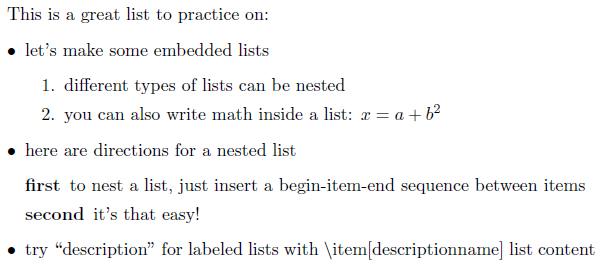
\includegraphics[width=\linewidth]{Ex_list}
\end{figure}

\end{frame}

\subsection{Page Margin}\label{Page Margin}
\begin{frame}\frametitle{Some Important Commands}
\rm
\fontsize{9pt}{11pt}\selectfont
\begin{itemize}
\item  For two column document class use: \textcolor[rgb]{0.98,0.00,0.00}{$\backslash$documentclass[twocolumn]\{article\}}\\[.20cm]

\item  If you want to make the article class two-sided: use \textcolor[rgb]{0.98,0.00,0.00}{$\backslash$documentclass[twoside]\{article\}}\\[.20cm]

\item To set the page size, add the following after \textcolor[rgb]{0.98,0.00,0.00}{$\backslash$documentclass}: \textcolor[rgb]{0.98,0.00,0.00}{$\backslash$usepackage\{geometry\}}\\[.20cm]
\textcolor[rgb]{0.98,0.00,0.00}{$\backslash$geometry\{a4paper\}}\\[.20cm]
    \begin{itemize}
      \item a0paper, a1paper, ..., a6paper,
      \item b0paper, b1paper, ..., b6paper,
      \item letterpaper,
      \item legalpaper,
      \item executivepaper
    \end{itemize}
\item For custom page size: \textcolor[rgb]{0.98,0.00,0.00}{$\backslash$geometry\{paperwidth=5.5in, paperheight=8.5in\}}
 \end{itemize}
\end{frame}

\begin{frame}\frametitle{Some Important Commands}
\rm
\fontsize{9pt}{11pt}\selectfont
\begin{itemize}
\item  To specifies the style of page numbers use: \textcolor[rgb]{0.98,0.00,0.00}{$\backslash$pagenumbering\{num\_style\}}\\[.20cm]
%%
\item Possible values of num\_style are:\\[.20cm]
%%
    \textbf{arabic}: Arabic numerals\\[.20cm]
    \textbf{roman}: Lowercase roman numerals\\[.20cm]
    \textbf{Roman}: Uppercase roman numerals\\[.20cm]
    \textbf{alph}: Lowercase letters\\[.20cm]
    \textbf{Alph}: Uppercase letters
\end{itemize}
\end{frame}



\begin{frame}\frametitle{Page Margin}
\rm
\fontsize{9pt}{11pt}\selectfont

\begin{columns}
	\begin{column}{6cm}
		\begin{figure}[h!]
			%\begin{center}
			%\centering
			\includegraphics[width=0.8\textwidth]{Latex_layout.eps}
			%\end{center}
		\end{figure}
	\end{column}
\begin{column}{4cm}
\footnotesize
\begin{enumerate}
	\item  $\backslash$hoffset
	\item  $\backslash$voffset
	\item $\backslash$oddsidemargin = 31pt
	\item $\backslash$topmargin = 20pt
	\item $\backslash$headheight = 12pt
	\item $\backslash$headsep = 25pt
	\item $\backslash$textheight = 592pt
	\item $\backslash$textwidth = 390pt
	\item $\backslash$marginparsep = 10pt
	\item $\backslash$marginparwidth = 35pt
	\item $\backslash$footskip = 30pt
\end{enumerate}

\begin{itemize}
	\item $\backslash$hoffset = 0pt
	\item $\backslash$voffset = 0pt
	\item  $\backslash$paperwidth = 597pt
	\item $\backslash$paperheight = 845pt
\end{itemize}

\end{column}
\end{columns}
\end{frame}



\begin{frame}\frametitle{Page Margin}
\rm
\fontsize{9pt}{11pt}\selectfont
\begin{center}
	\Huge \textcolor[rgb]{0.98,0.00,0.00}{!!USE TEMPLATES!!}
\end{center}
\end{frame}




%\section{Equation, Figures, and Tables}
\subsection{Equation, Figures, and Tables}

\begin{frame}{Math mode for writing equations}
Two ways in which one can write equations:

\begin{itemize}
	\item Use \$ Equation here \$ 
	\begin{itemize}
		\item Typically used inside a text or paragraph
	\end{itemize}
	\item Use $\backslash$begin\{equation\}\\ 
	write a single line equation here\\
	 $\backslash$end\{equation\}\\[0.7cm]
	 
	 Use package \textcolor[rgb]{0.98,0.00,0.00}{amsmath}\\[0.2cm]
	 \item Instead of equation other commands that can be used are: align, multiline etc.  
\end{itemize}
\end{frame}

\begin{frame}{Math mode for writing equations}
\textbf{Task:} Try these commands

$\backslash$hat\{x\}, $\backslash$tilde\{x\}, $\backslash$dot\{x\}, $\backslash$ddot\{x\} \\[0.6cm]

$\backslash$le ,$\backslash$ge, $\backslash$left[, $\backslash$right], $\backslash$left(, $\backslash$right) \\[1cm]

\textbf{Result:}

\hspace{2cm} \textcolor[rgb]{0.98,0.00,0.00}{$\hat{x}, \tilde{x}, \dot{x}, \ddot{x}, \le, \ge, \left[\right], \left(\right) $}
\end{frame} 


\begin{frame}{Math mode for writing equations}
\framesubtitle{Greek characters}
\begin{figure}
	\centering
	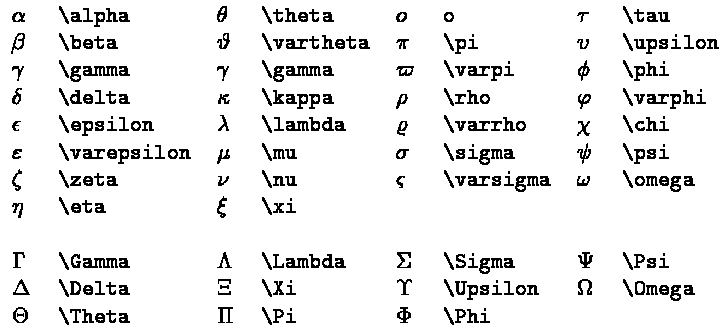
\includegraphics[width=\linewidth]{t1}
%	\caption{}
	\label{fig:t1}
	\end{figure}

Ref: \tiny \url{http://web.ift.uib.no/Teori/KURS/WRK/TeX/symALL.html}
\end{frame}


\begin{frame}{Math mode for writing equations}
\framesubtitle{Relation symbols}

\begin{figure}
	\centering
	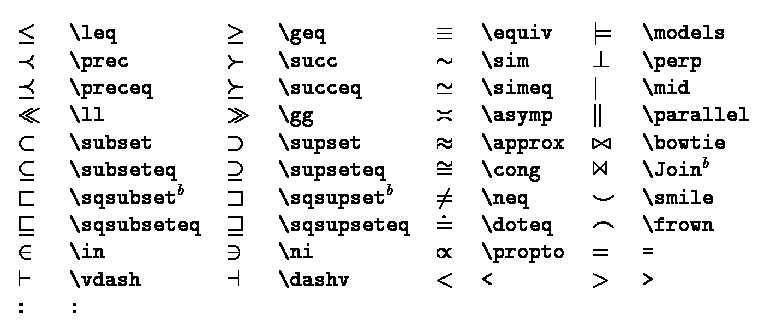
\includegraphics[width=\linewidth]{t3}
	\label{fig:t3}
\end{figure}
\end{frame}

\begin{frame}[fragile]\frametitle{Inserting Equation}
\rm
\fontsize{9pt}{11pt}\selectfont
\textcolor{red}{Example 1:}
\begin{verbatim}
\begin{equation}\label{eq:Addition}
a = b + c
\end{equation}

\end{verbatim}
\begin{figure}
	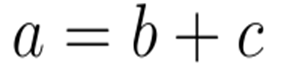
\includegraphics[height=0.5cm]{eq1.png}
\end{figure}
\textcolor{red}{Example 2:}
\begin{verbatim}
\begin{equation}\label{eq:Addition}
x^2 = y^3 + z_7
\end{equation}

\end{verbatim}
\begin{figure}
	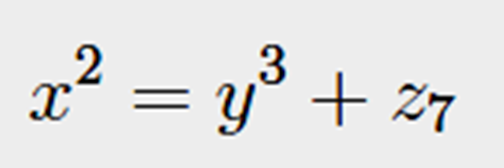
\includegraphics[height=0.7cm]{eq2.png}
\end{figure}
\end{frame}

\begin{frame}[fragile, plain]\frametitle{Inserting Equation}
\rm
\fontsize{9pt}{11pt}\selectfont
\textcolor{red}{Example 3:}
\begin{verbatim}
\begin{equation} \label{eq:Xbase}
x_2 = y_34 + z_{71} + a_83^ 94 +  b_{12}^{56}
\end{equation}


\end{verbatim}
\begin{figure}
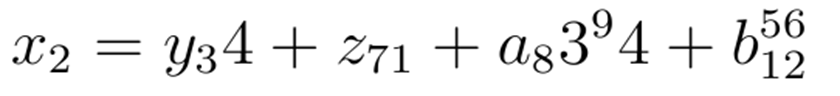
\includegraphics[height=0.5cm]{eq3.png}
\end{figure}
\textcolor{red}{Example 4:}
\begin{verbatim}
\begin{equation} \label{eq:SumOfSum}
S_{ij} = \frac{n}{100} \sum_{i}^ {10}  
\sum_{j}^{10} ( x_i + x_{ij} )
\end{equation}

\end{verbatim}
\begin{figure}
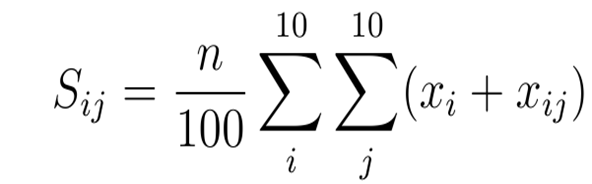
\includegraphics[height=0.9cm]{eq4.png}
\end{figure}
\end{frame}

\begin{frame}[fragile]\frametitle{No-number Equation}
\rm
\fontsize{9pt}{11pt}\selectfont
\textcolor{red}{Example 1:}
\begin{verbatim}
\begin{equation*}\label{eq:Addition}
a = b + c
\end{equation*}

\end{verbatim}
{\bf Note: } Insert mathematical expressions within text using \$ sign i.e. \$a+b\$
\end{frame}

\begin{frame}[fragile]{Additional features in a math mode}
\textcolor[rgb]{0.98,0.00,0.00}{$\backslash$begin\{align\}}: multi-line equations with alignment.
\newline

\begin{columns}
	\scriptsize
	\begin{column}{4cm}
		\textbf{Example:}
		
\begin{verbatim}
\begin{align} 
2x - 5y &=  8 \\ 
3x + 9y &=  -12
\end{align}
\end{verbatim} 
		
\begin{verbatim}
\begin{align*}
x&=y    &  w &=z  \\
2x&=-y  &  3w&=\frac{1}{2}z \\
-4 + 5x&=2+y &  w+2&=-1+w          
\end{align*}
\end{verbatim}
\end{column}

\begin{column}{4cm}
		\textbf{Output:}
		\begin{align} 
		2x - 5y &=  8 \\ 
		3x + 9y &=  -12
		\end{align}
		
		\begin{align*}
		x&=y           &  w &=z              \\
		2x&=-y         &  3w&=\frac{1}{2}z  \\
		-4 + 5x&=2+y   &  w+2&=-1+w          
		\end{align*}
	\end{column}
\end{columns}

\textcolor[rgb]{0.98,0.00,0.00}{$\backslash$nonumber}: removes numbers for an equations.
\end{frame}


\begin{frame}[containsverbatim]{Additional features in a math mode}
\textcolor[rgb]{0.98,0.00,0.00}{$\backslash$begin\{multiline\}}: command to enter long equations \\[0.4cm]
\begin{verbatim}
\begin{multline*}
p(x) = 3x^6 + 14x^5y + 590x^4y^2 + 19x^3y^3\\ 
- 12x^2y^4 - 12xy^5 + 2y^6 - a^3b^3
\end{multline*}
\end{verbatim} 
\begin{multline*}
p(x) = 3x^6 + 14x^5y + 590x^4y^2 + 19x^3y^3\\ 
- 12x^2y^4 - 12xy^5 + 2y^6 - a^3b^3
\end{multline*}
\end{frame}




\begin{frame}[fragile]\frametitle{Equations}
\rm
\textbf{Exercise 8. Equation writing}\\[.30cm]
\begin{itemize}
	\item Make a LaTeX file which produces the output shown in the pdf file \textbf{Ex8.pdf}
\end{itemize}
\end{frame}



%\subsection{Labelling Standards}
\begin{frame}[fragile]\frametitle{Labelling Standards}
\rm
\fontsize{9pt}{11pt}\selectfont

\begin{itemize}
	\item	For Equations 	:  	$\backslash$label\{{\bf eq:}Addition\}\\[.20cm]
	\item	For Tables \ \ \	 \		:	$\backslash$label\{{\bf table:}AnalysisResult\}\\[.20cm]
	\item	For Figure	\ \ \ \		: 	$\backslash$label\{{\bf fig:}Methodology\}\\[.20cm]
	\item	For Section	 \ \ \		:$\backslash$label\{{\bf	sec:}Methodology\}\\[.20cm]
	
	
\end{itemize}

\end{frame}


%\subsection{Tables}

\begin{frame}[fragile]\frametitle{Inserting Tables}
\rm
\fontsize{9pt}{11pt}\selectfont
{\color{red}
\begin{verbatim}
\begin{tablular}{ l c r p }

Table contents

\end{tabular}
\end{verbatim}
}
\begin{itemize}
\item Four columns table\\[.20cm]
\item {\bf \textcolor{red}{l} for left, \textcolor{red}{c} for center, \textcolor{red}{r} for right, \textcolor{red}{p} for paragraph}\\[.20cm]
\end{itemize}

\end{frame}

\begin{frame}\frametitle{Inserting Tables}
\rm
\fontsize{9pt}{11pt}\selectfont
Example 1:
\begin{figure}
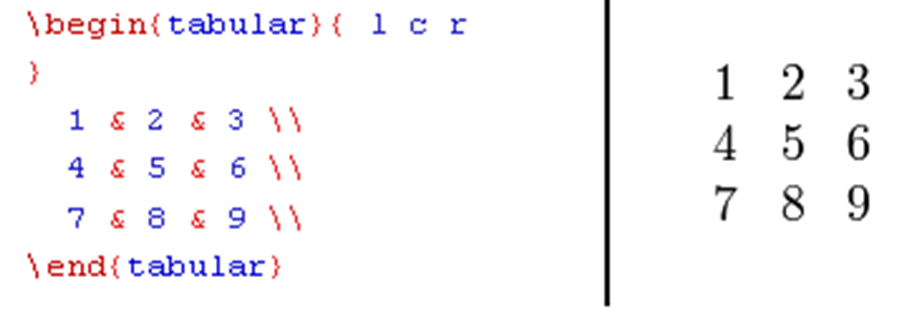
\includegraphics[height=2.5cm]{tb1.png}
\end{figure}
Example 2:
\begin{figure}
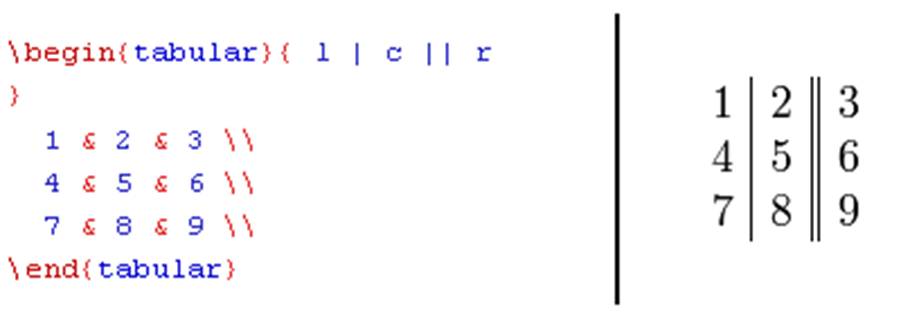
\includegraphics[height=2.5cm]{tb2.png}
\end{figure}
\end{frame}

\begin{frame}\frametitle{Inserting Tables}
\rm
\fontsize{9pt}{11pt}\selectfont
Example 3:
\begin{figure}
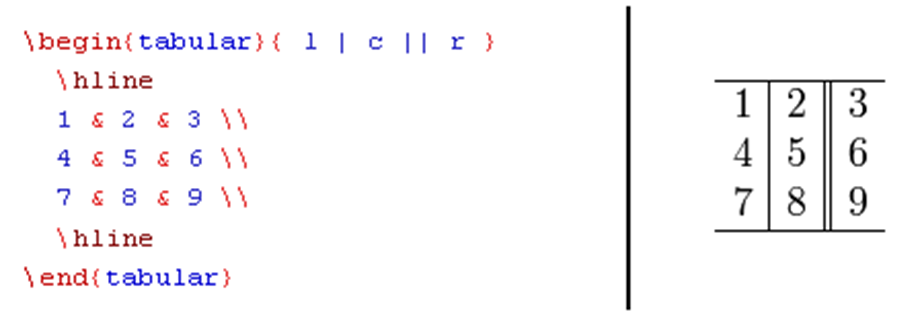
\includegraphics[height=2.5cm]{tb3.png}
\end{figure}
Example 4:
\begin{figure}
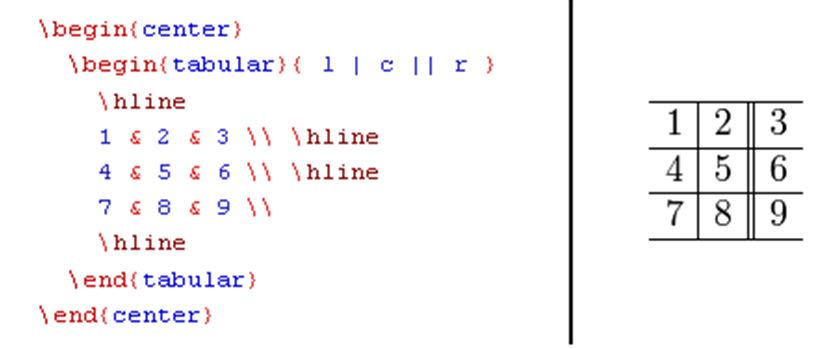
\includegraphics[height=2.5cm]{tb4.png}
\end{figure}
\end{frame}

\begin{frame}\frametitle{Inserting Tables}
\rm
\fontsize{9pt}{11pt}\selectfont
Example 5:
\begin{figure}
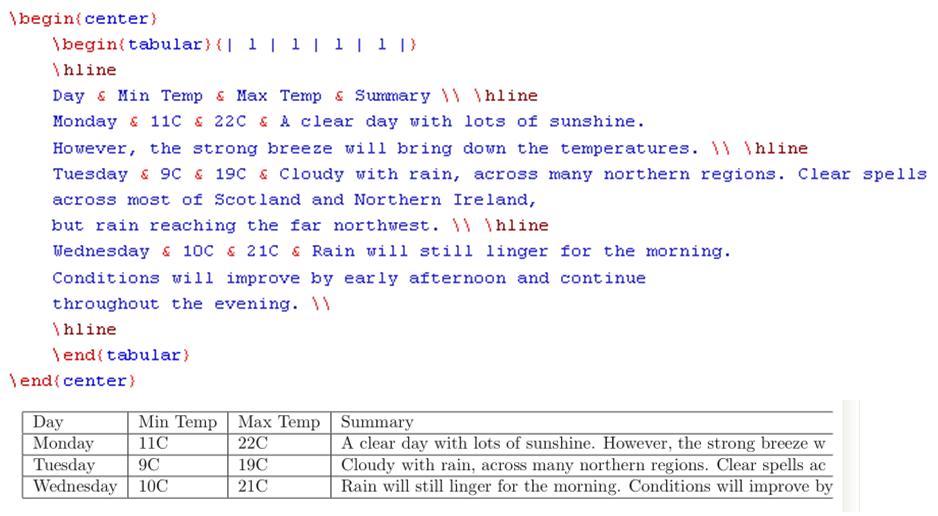
\includegraphics[height=6cm]{tb5.png}
\end{figure}

\end{frame}

\begin{frame}\frametitle{Inserting Tables}
\rm
\fontsize{9pt}{11pt}\selectfont
Example 6:
\begin{figure}
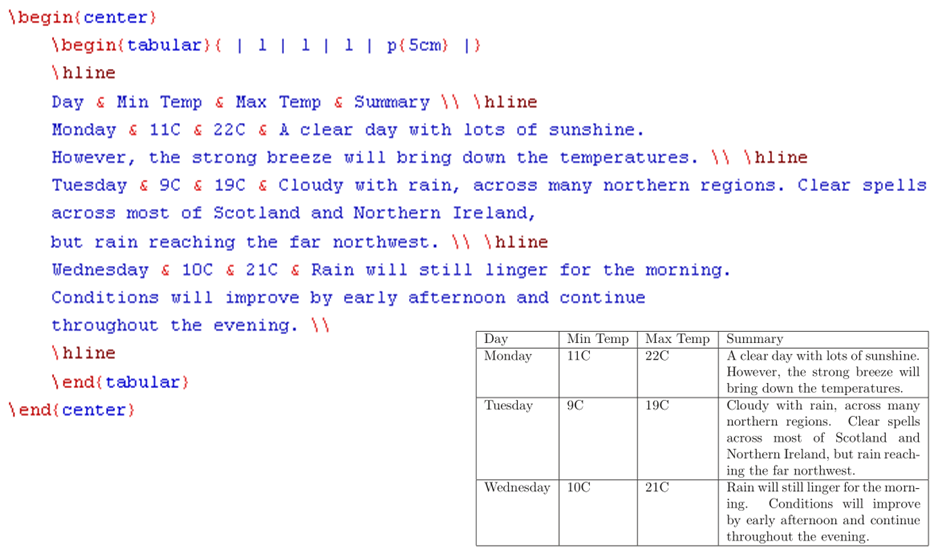
\includegraphics[height=6cm]{tb6.png}
\end{figure}

\end{frame}

\begin{frame}\frametitle{Inserting Tables}
\rm
\fontsize{9pt}{11pt}\selectfont
Example 7:
\begin{figure}
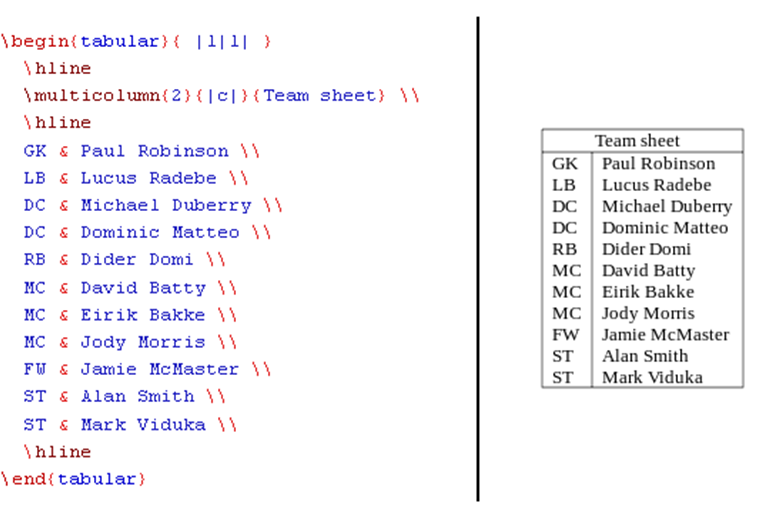
\includegraphics[height=6cm]{tb7.png}
\end{figure}

\end{frame}

\begin{frame}\frametitle{Adding Caption to Tables}
\rm
\fontsize{9pt}{11pt}\selectfont
{\color{blue}$\backslash$begin\{table\} } \\[.30cm]
\  \  \ {\color{green}$\backslash$begin\{tablular\}\{ l c r p \}\\[.30cm]
\  \  \ $\backslash$end\{tabular\}  }\\[.30cm]
\  \  \ {\color{red}$\backslash$caption\{\}\\[.30cm]
\  \  \ $\backslash$label\{\}}\\[.30cm]
{\color{blue}$\backslash$end\{table\}}


\end{frame}

\begin{frame}{Tables}
\textbf{Exercise 10(a). Making Tables}\\[.30cm]
\begin{itemize}
	\item Write Latex code which produces following output.
\end{itemize}
\begin{figure}
	\centering
	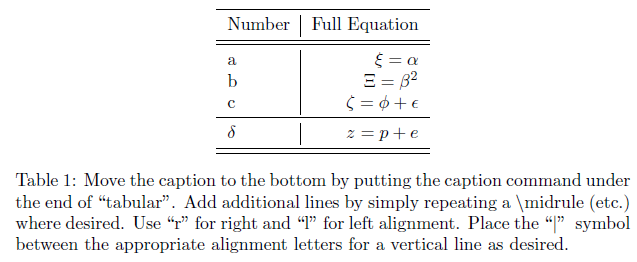
\includegraphics[width=\linewidth]{Ex8}
	
	\label{fig:ex8}
\end{figure}
\end{frame}



\begin{frame}{Tables}
\textbf{Exercise 10(b). Making Tables}\\[.30cm]
\begin{itemize}
	\item Write Latex code which produces following output.
\end{itemize}
\begin{table}[htbp]
	\caption{Table Type Styles}
	\begin{center}
		\begin{tabular}{|c|c|c|c|}
			\hline
			\textbf{Table}&\multicolumn{3}{|c|}{\textbf{Table Column Head}} \\
			\cline{2-4} 
			\textbf{Head} & \textbf{\textit{Table column subhead}}& \textbf{\textit{Subhead}}& \textbf{\textit{Subhead}} \\
			\hline
			copy& More table copy$^{\mathrm{a}}$& &  \\
			\hline
			\multicolumn{4}{c}{$^{\mathrm{a}}$Sample of a Table footnote.}
		\end{tabular}
		\label{tab1}
	\end{center}
\end{table}
\end{frame}


\begin{frame}[fragile]\frametitle{Inserting Figures}
\rm
\fontsize{9pt}{11pt}\selectfont

\begin{verbatim}
Add Package:  \usepackage{graphicx}
\end{verbatim}
Example 1:
{\color{red}
\begin{verbatim}
\begin{figure}
\includegraphics{FiguresName} % figure
\caption{Result}  %Caption
\label{fig:Result}  %Label
\end{figure}
\end{verbatim}
}
Example 2:
{\color{red}
\begin{verbatim}
\begin{figure}
\includegraphics[height=3cm, width=3cm]{FiguresName} % figure
\caption{Result}  %Caption
\label{fig:Result}  %Label
\end{figure}
\end{verbatim}
}
\end{frame}


\begin{frame}[fragile]{Subfigures}
\begin{verbatim}
Add Package:  \usepackage{subfigure}
\end{verbatim}
\scriptsize
Example 1:
{\color{blue}
\begin{verbatim}
\begin{figure}
\subfigure[Subfigure 1]
{\includegraphics[height=3cm,width=3cm]{Koala.jpg}}~~~~
\subfigure[Subfigure 2]
{\includegraphics[height=3cm,width=3cm]{Penguins.jpg}}
\caption{Result}  %Caption
\label{fig:Result}  %Label
\end{figure}
\end{verbatim}
}

\begin{figure}
\subfigure[Subfigure 1]{\includegraphics[height=1.5cm, width=2cm]{Koala.jpg}}~~~~\subfigure[Subfigure 2]{\includegraphics[height=1.5cm, width=2cm]{Penguins.jpg}}
	\caption{Result}  %Caption
	\label{fig:Result}  %Label
\end{figure}
\end{frame}

\begin{frame}{Inserting figures in document}
\textbf{Exercise 11. Making Figures}\\[.30cm]
\begin{itemize}
	\item Write Latex code for the content given in \textbf{Ex11- figures.pdf}.
\end{itemize}


\end{frame}

%\begin{frame}{More on Figure}
%\framesubtitle{Subfigures}
%content...
%\end{frame}
%
%\begin{frame}{Exercise 12 on subfigure}
%content...
%\end{frame}

\begin{frame}\frametitle{\LaTeX}
\rm
\fontsize{9pt}{11pt}\selectfont
\begin{center}
\Huge \textcolor[rgb]{0.98,0.00,0.00}{!!Compile \& Run Multiple Times!!}\\
Dealing with large documents

\end{center}
\end{frame}

\subsection{Package Manager}
\begin{frame}\frametitle{Environment Setup}
\rm
\fontsize{9pt}{11pt}\selectfont
\begin{center}
\Large Internet Setting and error handling for  \textcolor[rgb]{0.98,0.00,0.00}{Packages}\\[0.4cm]

\LARGE !!.. Demonstration ..!! 

 

\end{center}
\end{frame}

%\begin{frame}\frametitle{Environment Setup-Step 1}
%\rm
%\fontsize{9pt}{11pt}\selectfont
%\begin{center}
%\bf Start $-->$ MileTex $-->$ Maintenance  $-->$ Package Manager 
%\begin{figure}
%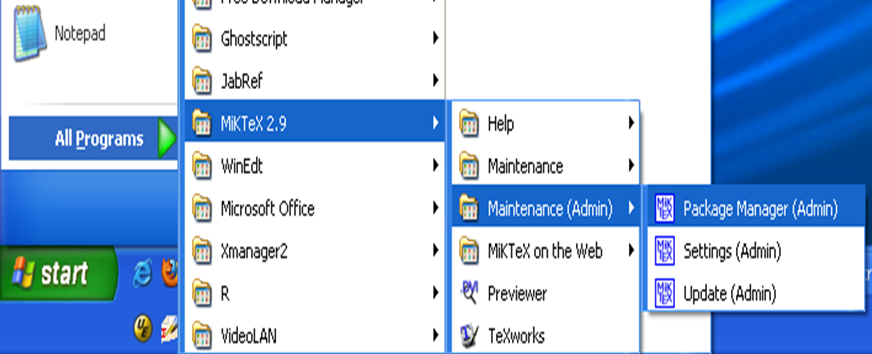
\includegraphics[height=4cm]{env1.png}
%\end{figure}
%
%\end{center}
%\end{frame}
%
%\begin{frame}\frametitle{Environment Setup-Step 2}
%\rm
%\fontsize{9pt}{11pt}\selectfont
%\begin{center}
%\bf Repository $-->$ Change Package Repository 
%\begin{figure}
%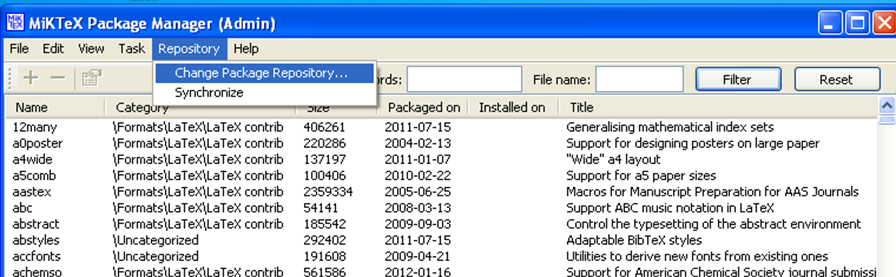
\includegraphics[height=3cm]{env2.png}
%\end{figure}
%
%\end{center}
%\end{frame}
%
%\begin{frame}\frametitle{Environment Setup-Step 3}
%\rm
%\fontsize{9pt}{11pt}\selectfont
%\begin{center}
%\bf Packages shall be \dots  $-->$ Connection Settings\dots $-->$Proxy Setting
%\begin{figure}
%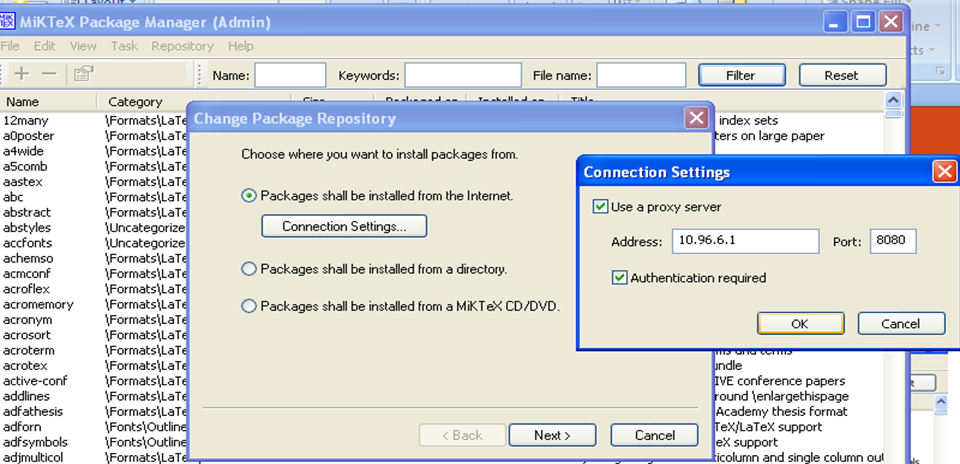
\includegraphics[height=4cm]{env3.png}
%\end{figure}
%
%\end{center}
%\end{frame}
%
%\begin{frame}\frametitle{Environment Setup}
%\rm
%\fontsize{9pt}{11pt}\selectfont
%\begin{center}
%\Huge  \textcolor[rgb]{0.98,0.00,0.00}{!!Environment is Set!!}
%
%\end{center}
%\end{frame}



\section{References}
\subsection{Inserting References}
\begin{frame}\frametitle{Inserting References}
\rm
\fontsize{9pt}{11pt}\selectfont
\begin{itemize}
\item Insert  following two commands at the end of document, before \textbf{$\backslash$end\{document\}}\\[.30cm]
\item Simplest way to make bibliography file is by using \textcolor{red}{JabRef}\\[.30cm]
\end{itemize}
{\bf $\backslash$bibliographystyle\{{\color{red}plain}\}\\[.30cm]
$\backslash$bibliography\{{\color{red}references}\}}
\end{frame}
%\subsection{JabRef}
%
%\begin{frame}[fragile]\frametitle{Inserting References}
%\rm
%\fontsize{9pt}{11pt}\selectfont
%\begin{figure}
%
\includegraphics[height=5cm]{ref1.png}
%\end{figure}
%
%\end{frame}

%%%%%%%%%%%%%%%%%%%%%%%%%%%%%%%%%%%%%%%%%%%%%%%

\subsection{Installing JabRef on Windows}
\begin{frame}{JabRef on Windows}%{Optional Subtitle}
\begin{figure}
\subfigure[Step 1: Download the JabRef: http://www.jabref.org/.]{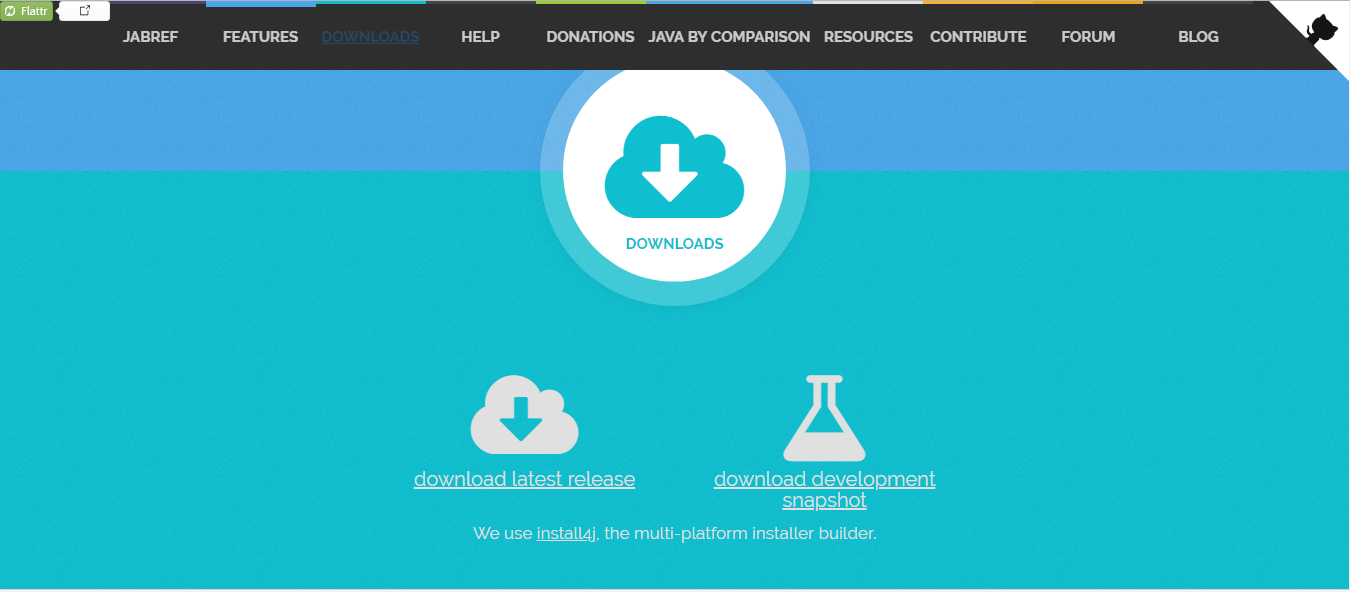
\includegraphics[width=0.5\textwidth,height=0.5\textheight]{fig39.png}}
\end{figure}

\end{frame}

\begin{frame}{JabRef on Windows}%{Optional Subtitle}
\begin{itemize}
\item Step 2: Install/update Java Runtime Environment
\end{itemize}
\end{frame}

\begin{frame}{JabRef on Windows}%{Optional Subtitle}

\begin{figure}
\subfigure[Step 3: Install the JabRef.]{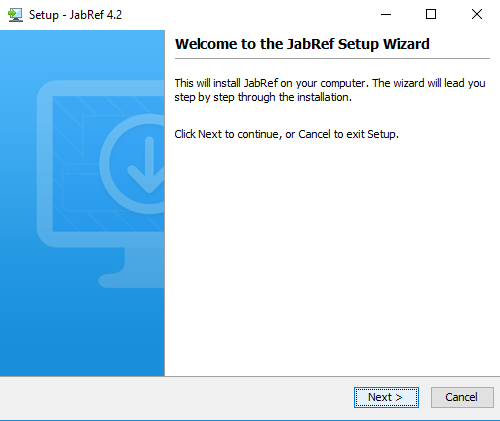
\includegraphics[width=0.5\textwidth,height=0.5\textheight]{fig9.png}}
\end{figure}

\end{frame}

\begin{frame}{JabRef on Windows}%{Optional Subtitle}

\begin{figure}
\subfigure[Step 4: Open the JabRef and create new JabRef file by clicking the top-left symbol.]{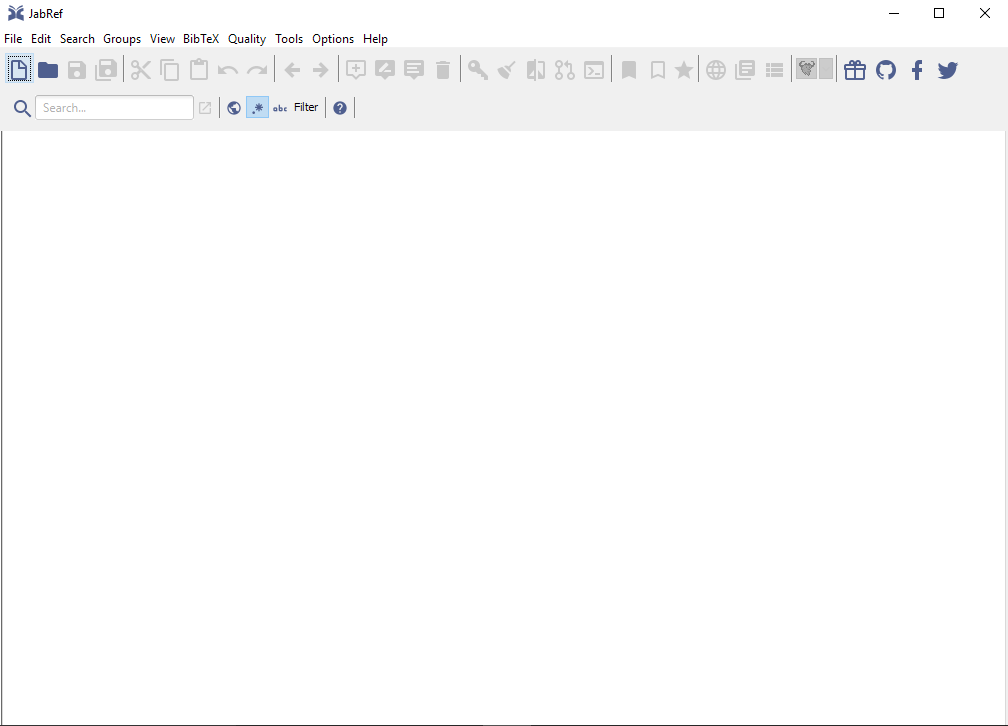
\includegraphics[width=0.5\textwidth,height=0.5\textheight]{fig10.png}}
\end{figure}

\end{frame}

\begin{frame}{JabRef on Windows}%{Optional Subtitle}

\begin{figure}
\subfigure[Step 5: If on network, setup the connection settings by selecting the preferences.]{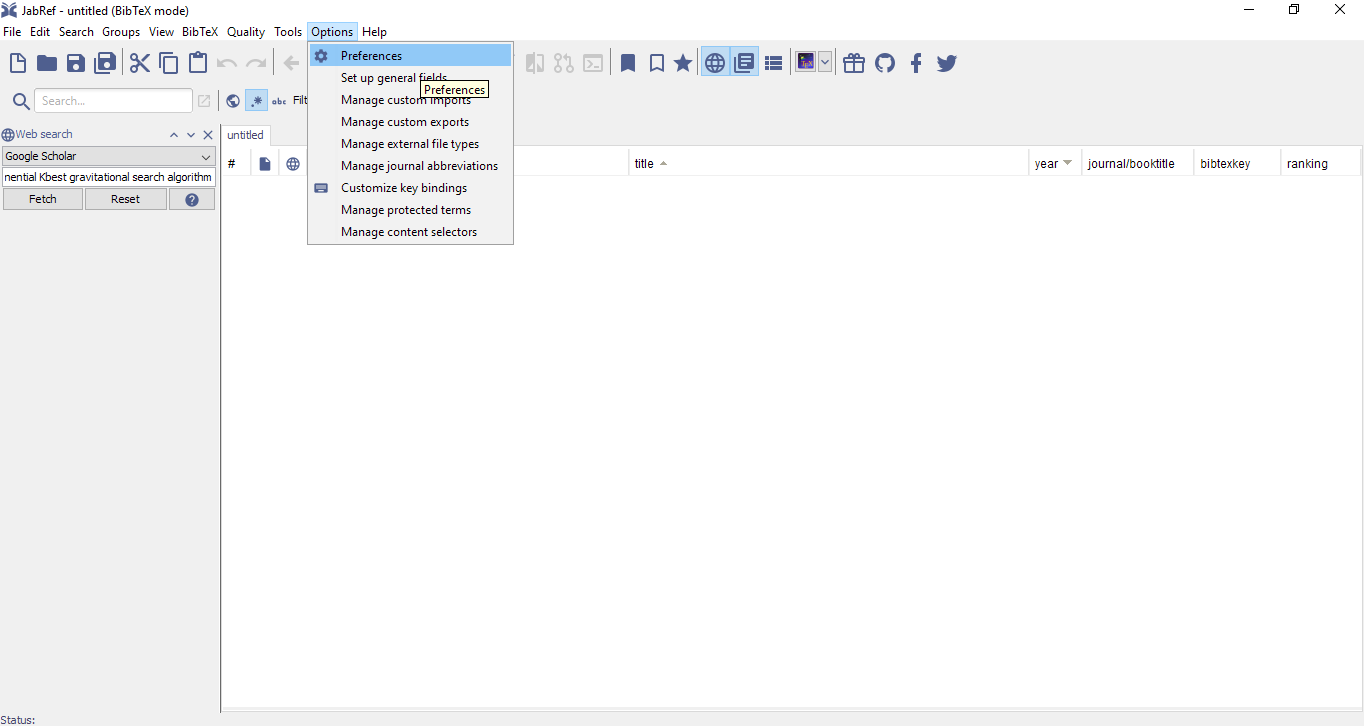
\includegraphics[width=0.5\textwidth,height=0.5\textheight]{fig41.png}}
\end{figure}

\end{frame}

\begin{frame}{JabRef on Windows}%{Optional Subtitle}

\begin{figure}
\subfigure[Step 6: Select \lq Network \rq option and the required details.]{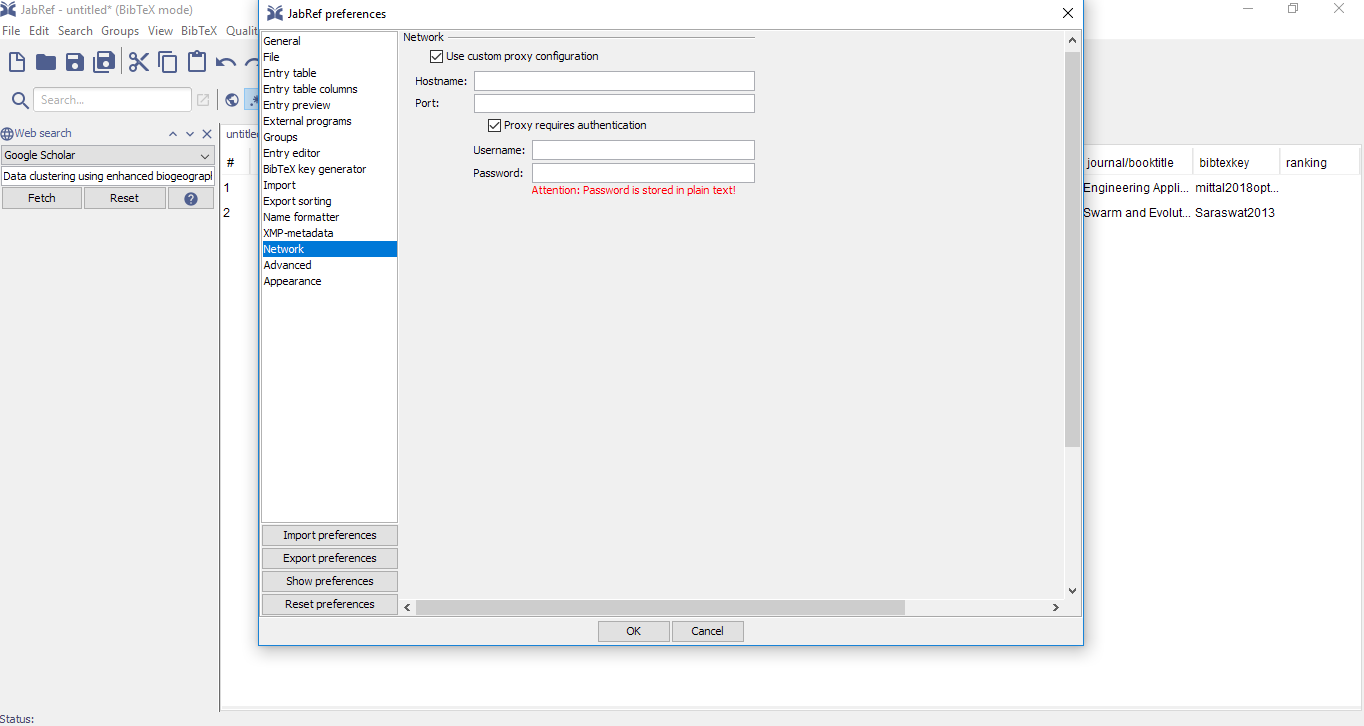
\includegraphics[width=0.5\textwidth,height=0.5\textheight]{fig40.png}}
\end{figure}

\end{frame}

\begin{frame}{JabRef on Windows}%{Optional Subtitle}
\begin{itemize}
\item Generally, BibTex key of paper can be generated in three ways:
\begin{itemize}
\item Manually
\item Using DOI
\item Using Paper name
\end{itemize}
\end{itemize}


\end{frame}


\begin{frame}{JabRef on Windows}{$1^{st}$ way: Manual}

\begin{figure}
	
\subfigure[Step 1: Click on $+$ symbol.]{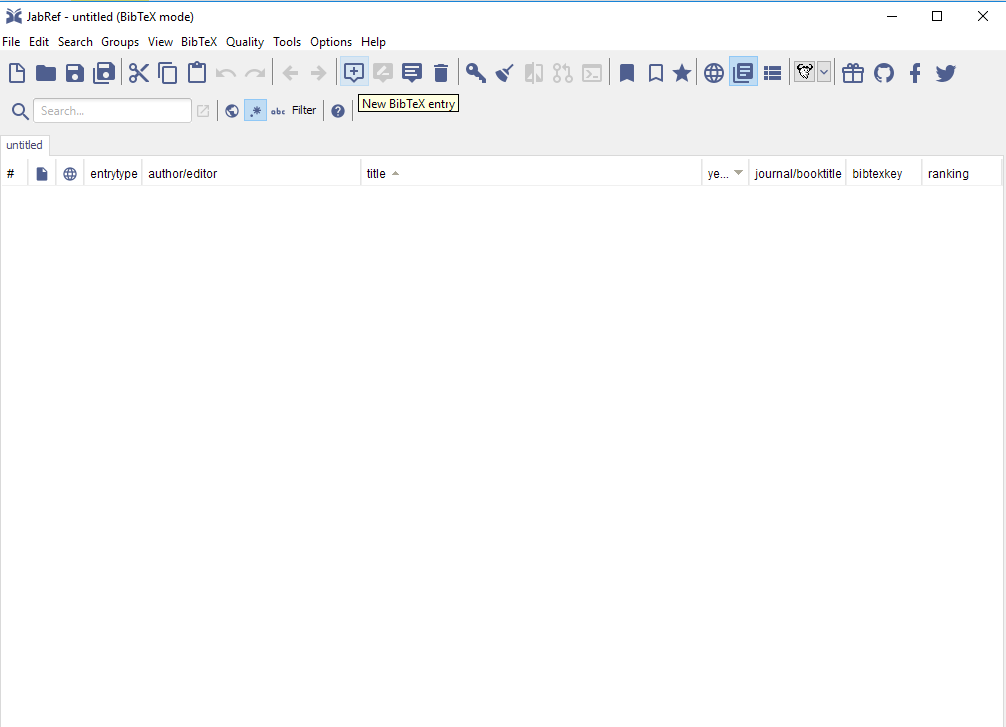
\includegraphics[width=0.5\textwidth,height=0.5\textheight]{fig11.png}}
\caption{}
\end{figure}

\end{frame}

\begin{frame}{JabRef on Windows}{$1^{st}$ way: Manual}

\begin{figure}
\subfigure[Step 2: Select \lq Article \rq on the popup window.]{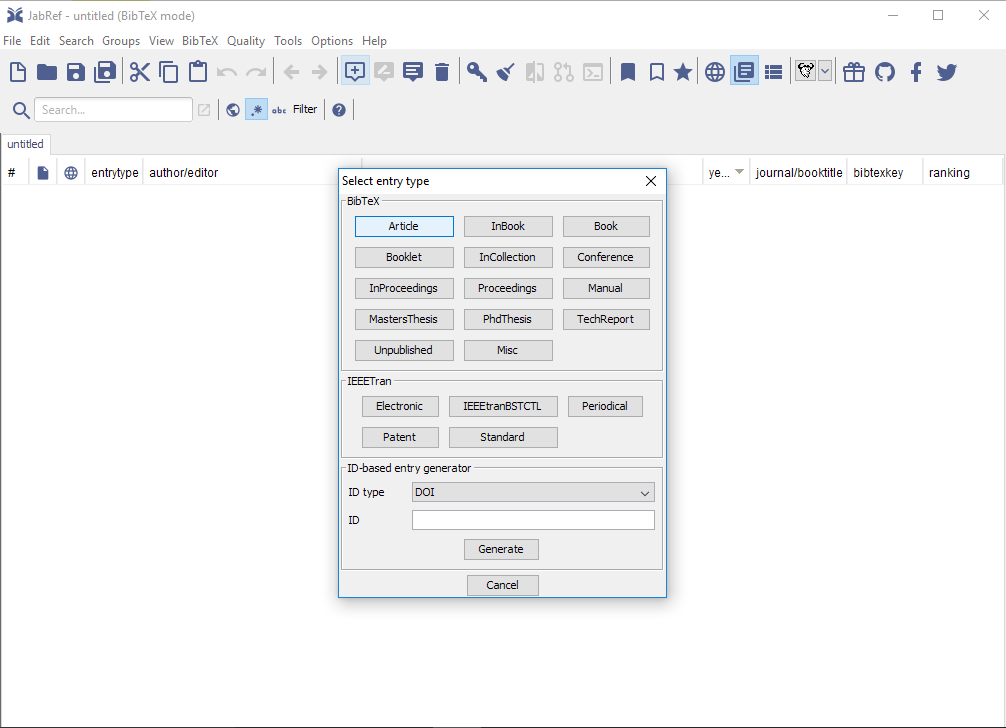
\includegraphics[width=0.5\textwidth,height=0.5\textheight]{fig12.png}}
\end{figure}

\end{frame}




\begin{frame}{JabRef on Windows}{$1^{st}$ way: Manual}

\begin{figure}
\subfigure[Step 3: Window will be like this.]{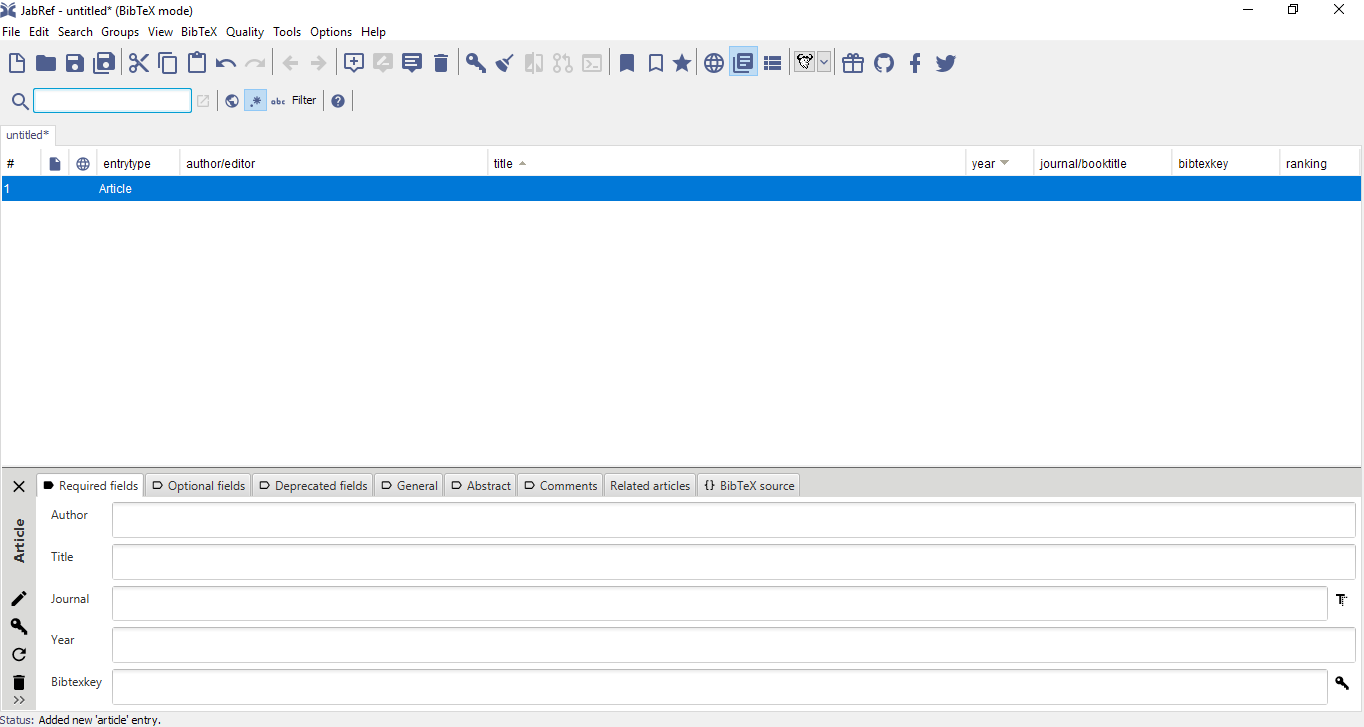
\includegraphics[width=0.5\textwidth,height=0.5\textheight]{fig13.png}}
\end{figure}

\end{frame}

\begin{frame}{JabRef on Windows}{$1^{st}$ way: Manual}

\begin{figure}
\subfigure[Step 4: Fetch the BibTex key online.]{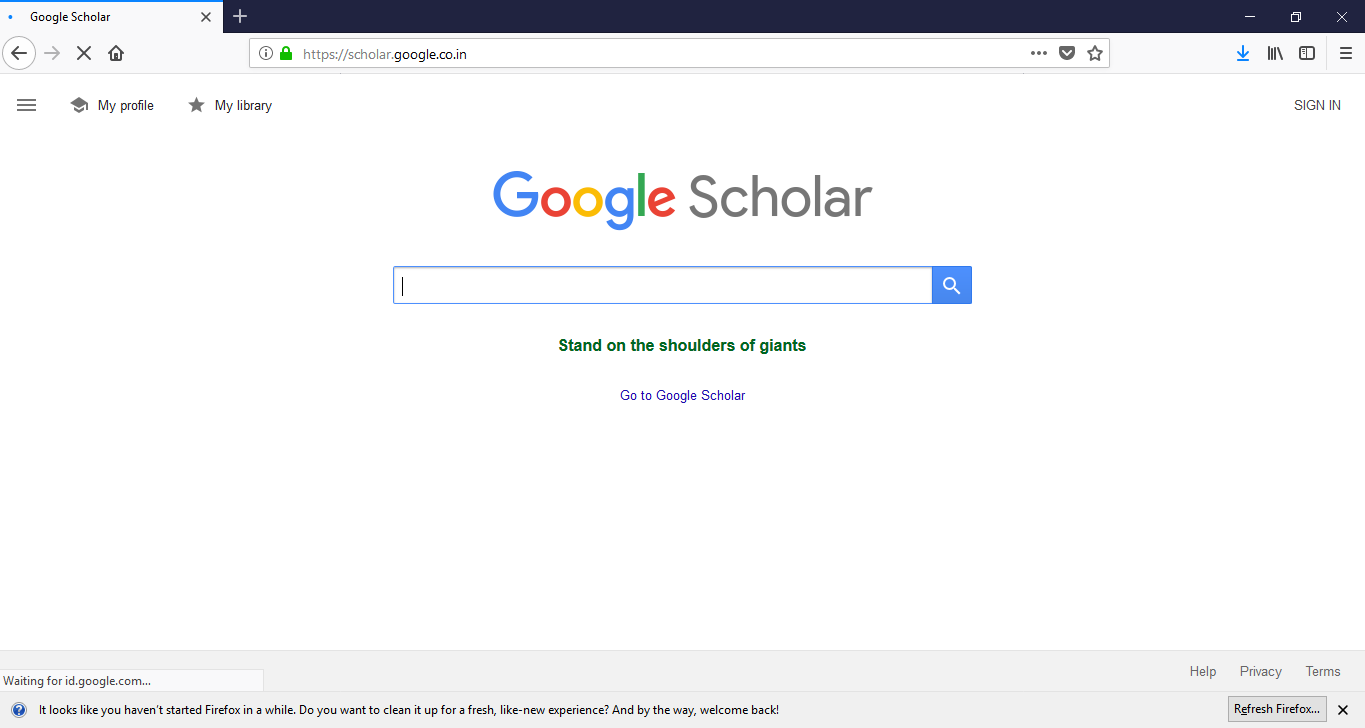
\includegraphics[width=0.5\textwidth,height=0.5\textheight]{fig14.png}}
\end{figure}

\end{frame}

\begin{frame}{JabRef on Windows}{$1^{st}$ way: Manual}

\begin{figure}
\subfigure[Step 5: Click on the \lq Cite\rq.]{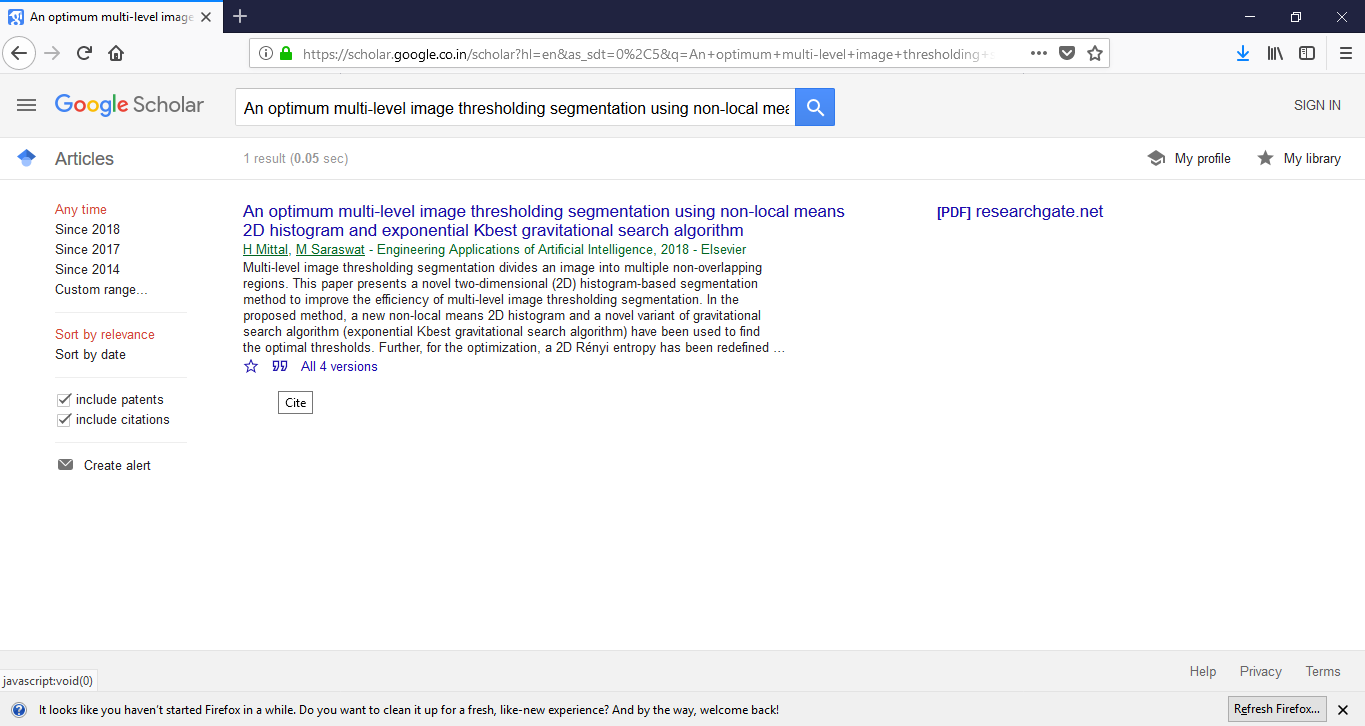
\includegraphics[width=0.5\textwidth,height=0.5\textheight]{fig15.png}}
\end{figure}

\end{frame}


\begin{frame}{JabRef on Windows}{$1^{st}$ way: Manual}

\begin{figure}
\subfigure[Step 6: Click on the \lq BibTex\rq.]{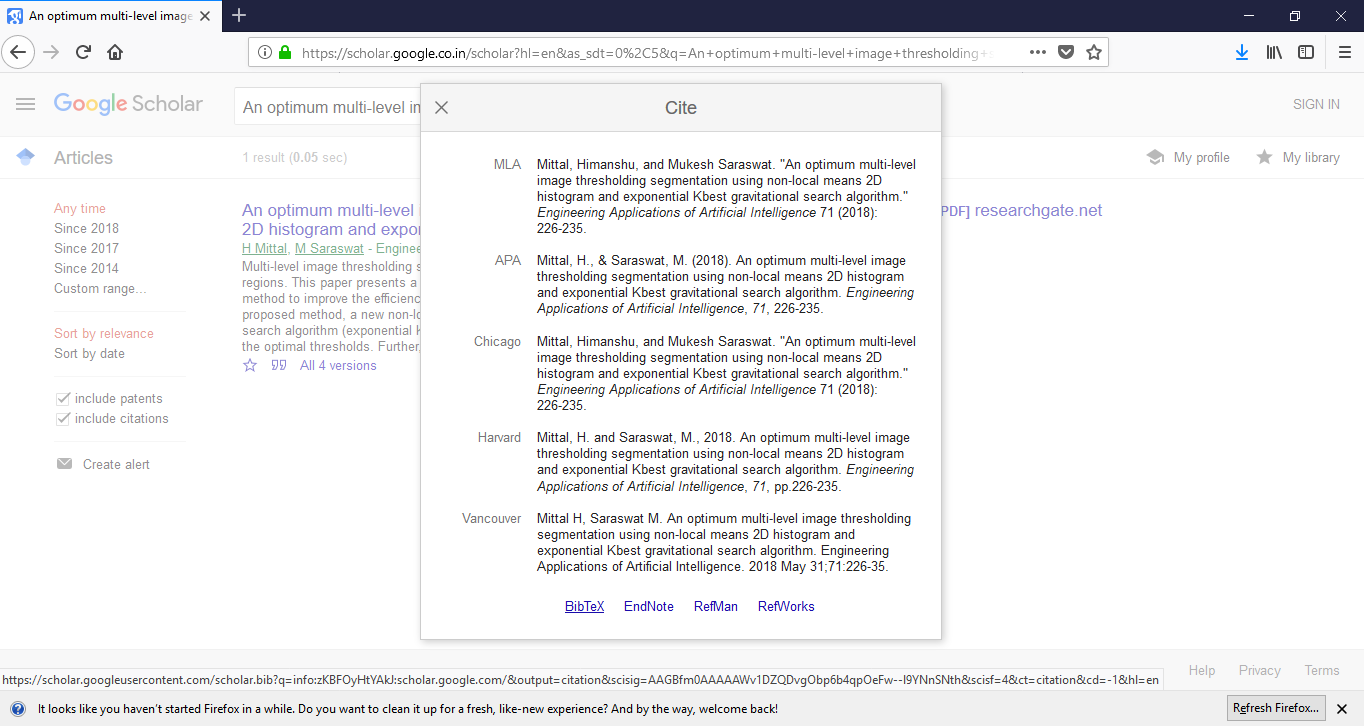
\includegraphics[width=0.5\textwidth,height=0.5\textheight]{fig16.png}}
\end{figure}

\end{frame}

\begin{frame}{JabRef on Windows}{$1^{st}$ way: Manual}

\begin{figure}
\subfigure[Step 7a: Select the BibTex content.]{\includegraphics[width=0.5\textwidth,height=0.5\textheight]{fig17.png}}~~~~\subfigure[Step 7b: Copy the BibTex content.]{\includegraphics[width=0.5\textwidth,height=0.5\textheight]{fig18.png}}
%\caption{[]}
\end{figure}

\end{frame}


\begin{frame}{JabRef on Windows}{$1^{st}$ way: Manual}

\begin{figure}
\subfigure[Step 8: Go to JabRef window, click the \lq BibTex source \rq tab, and paste the copied text.]{\includegraphics[width=0.5\textwidth,height=0.5\textheight]{fig19.png}}
\end{figure}

\end{frame}

\begin{frame}{JabRef on Windows}{$1^{st}$ way: Manual}

\begin{figure}
\subfigure[Step 9: Check the entries, if required to.]{\includegraphics[width=0.5\textwidth,height=0.5\textheight]{fig20.png}}
\caption{}
\end{figure}

\end{frame}




\begin{frame}{JabRef on Windows}{$2^{nd}$ way: DOI}

\begin{figure}
\subfigure[Step 1: Go to the paper online.]{\includegraphics[width=0.5\textwidth,height=0.5\textheight]{fig23.png}}
\end{figure}

\end{frame}

\begin{frame}{JabRef on Windows}{$2^{nd}$ way: DOI}

\begin{figure}
\subfigure[Step 2: Copy the \lq DOI \rq of the paper.]{\includegraphics[width=0.5\textwidth,height=0.5\textheight]{fig24.png}}
\end{figure}

\end{frame}

\begin{frame}{JabRef on Windows}{$2^{nd}$ way: DOI}

\begin{figure}
\subfigure[Step 3: Click on $+$ symbol.]{\includegraphics[width=0.5\textwidth,height=0.5\textheight]{fig11.png}}
\end{figure}

\end{frame}

\begin{frame}{JabRef on Windows}{$2^{nd}$ way: DOI}

\begin{figure}
\subfigure[Step 4: Entry the \lq DOI \rq of the paper  at the bottom of the popup window.]{\includegraphics[width=0.5\textwidth,height=0.5\textheight]{fig25.png}}
\end{figure}

\end{frame}

\begin{frame}{JabRef on Windows}{$2^{nd}$ way: DOI}

\begin{figure}
\subfigure[Step 5: JafRef will have the entry like this.]{\includegraphics[width=0.5\textwidth,height=0.5\textheight]{fig26.png}}
\caption{}
\end{figure}

\end{frame}

\begin{frame}{JabRef on Windows}{$3^{rd}$ way: DOI}

\begin{figure}
\subfigure[Step 1: Copy the paper name]{\includegraphics[width=0.5\textwidth,height=0.5\textheight]{fig27.png}}
\end{figure}

\end{frame}


\begin{frame}{JabRef on Windows}{$3^{rd}$ way: DOI}

\begin{figure}
\subfigure[Step 2: Click on the web search option.]{\includegraphics[width=0.5\textwidth,height=0.5\textheight]{fig28.png}}
\end{figure}

\end{frame}

\begin{frame}{JabRef on Windows}{$3^{rd}$ way: DOI}

\begin{figure}
\subfigure[Step 3: Select the appropriate web source.]{\includegraphics[width=0.5\textwidth,height=0.5\textheight]{fig29.png}}
\end{figure}

\end{frame}

\begin{frame}{JabRef on Windows}{$3^{rd}$ way: DOI}

\begin{figure}
\subfigure[Step 4: Enter the paper name and click \lq Fetch \rq.]{\includegraphics[width=0.5\textwidth,height=0.5\textheight]{fig30.png}}
\end{figure}

\end{frame}

\begin{frame}{JabRef on Windows}{$3^{rd}$ way: DOI}

\begin{figure}
\subfigure[Step 5: Click \lq Generate Now \rq after selecting the appropriate paper.]{\includegraphics[width=0.5\textwidth,height=0.5\textheight]{fig31.png}}
\end{figure}

\end{frame}

\begin{frame}{JabRef on Windows}{$3^{rd}$ way: DOI}

\begin{figure}
\subfigure[Step 6: Click \lq OK \rq .]{\includegraphics[width=0.5\textwidth,height=0.5\textheight]{fig32.png}}
\caption{}
\end{figure}

\end{frame}


\subsection{Entering BibTex key in Paper}
\begin{frame}{BibTex key in Paper}%{3^{rd} way: DOI}
\begin{itemize}
\item There are two ways to enter the BibTex key in paper:
\begin{itemize}
\item Manually
\item Push: Can't use with MikTex
\end{itemize}
\end{itemize}

\end{frame}

\begin{frame}{BibTex key in Paper}{$1^{st}$ way: Manual}

\begin{figure}
\subfigure[Step 1.1: Right\-click the required entry in JabRef, select the highlighted option, and paste in the desired location in paper.]{\includegraphics[width=0.5\textwidth,height=0.5\textheight]{fig21.png}}
\end{figure}

\end{frame}

\begin{frame}{BibTex key in Paper}{$2^{nd}$ way: Push}

\begin{figure}
\subfigure[Step 2.1: Place the mouse cursor at desired location in paper and select the \lq Push \rq in JabRef.]{\includegraphics[width=0.5\textwidth,height=0.5\textheight]{fig34.png}}
\end{figure}

\end{frame}

\begin{frame}{BibTex key in Paper}{$2^{nd}$ way: Push}

\begin{figure}
\subfigure[Step 2.2: In JabRef, other IDE can be selected too.]{\includegraphics[width=0.5\textwidth,height=0.5\textheight]{fig33.png}}
\end{figure}

\end{frame}

\subsection{Saving the JabRef File}
\begin{frame}{Saving BibTex File}%{3^{rd} way: DOI}
\begin{itemize}
\item Click the \lq save \rq symbol in JabRef.
\item Select the location and name of the BibTex File.
\item A file of entered name with \lq .bib \rq extension will be created in the selected location.
\item Remember: the $*$ on the name of the JabRef file means changes are not saved.
\end{itemize}

\end{frame}








%\begin{frame}\frametitle{Inserting References}
%\rm
%\fontsize{9pt}{11pt}\selectfont
%\begin{figure}
%\includegraphics[height=5cm]{ref2.png}
%\end{figure}
%
%\end{frame}
%
%\begin{frame}\frametitle{Inserting References}
%\rm
%\fontsize{9pt}{11pt}\selectfont
%\begin{figure}
%\includegraphics[height=5cm]{ref3.png}
%\end{figure}
%
%\end{frame}
%
%\begin{frame}\frametitle{Inserting References}
%\rm
%\fontsize{9pt}{11pt}\selectfont
%\begin{figure}
%\includegraphics[height=5cm]{ref4.png}
%\end{figure}
%
%\end{frame}
%
%\begin{frame}\frametitle{Inserting References}
%\rm
%\fontsize{9pt}{11pt}\selectfont
%\begin{figure}
%\includegraphics[height=5cm]{ref5.png}
%\end{figure}
%
%\end{frame}
%
%\begin{frame}\frametitle{Inserting References}
%\rm
%\fontsize{9pt}{11pt}\selectfont
%\begin{figure}
%\includegraphics[height=4.5cm]{ref6.png}
%\end{figure}
%
%\end{frame}
%
%\begin{frame}\frametitle{Inserting References}
%\rm
%\fontsize{9pt}{11pt}\selectfont
%\begin{figure}
%\includegraphics[height=5cm]{ref7.png}
%\end{figure}
%
%\end{frame}
%
%\begin{frame}\frametitle{Inserting References}
%\rm
%\fontsize{9pt}{11pt}\selectfont
%\begin{figure}
%\includegraphics[height=5cm]{ref8.png}
%\end{figure}
%
%\end{frame}
%
%\begin{frame}\frametitle{Inserting References}
%\rm
%\fontsize{9pt}{11pt}\selectfont
%\begin{figure}
%\includegraphics[height=5cm]{ref9.png}
%\end{figure}
%
%\end{frame}
%
%\begin{frame}\frametitle{Inserting References}
%\rm
%\fontsize{9pt}{11pt}\selectfont
%\begin{figure}
%\includegraphics[height=5cm]{ref10.png}
%\end{figure}
%
%\end{frame}
%
%\begin{frame}\frametitle{Inserting References}
%\rm
%\fontsize{9pt}{11pt}\selectfont
%\begin{figure}
%\includegraphics[height=5cm]{ref11.png}
%\end{figure}
%
%\end{frame}
%
%\begin{frame}\frametitle{Inserting References}
%\rm
%\fontsize{9pt}{11pt}\selectfont
%\begin{figure}
%\includegraphics[height=5cm]{ref12.png}
%\end{figure}
%\begin{center}{\color{red} !!Check the References!!}\end{center}
%\end{frame}


\begin{frame}{Learning by doing}
\textbf{Exercise 13:}
\begin{itemize}
	\item Using  Google Scholar (scholar.google.com), search for the following: \lq\lq An optimum multi-level image thresholding segmentation using non-local means 2D histogram and exponential Kbest gravitational search algorithm \rq\rq
	\item Note the top hitting article, click on \textbf{cite} at the bottom of the entry, and click on \textbf{bibtex} at the bottom of the pop up window.
	\item Copy and paste the information into a new file called \textbf{mybib$\cdot$bib}.
\end{itemize}

\end{frame}



%\section{Thesis writing}
%\subsection{Document class}\label{Document class}
%\begin{frame}{The document class}
%\begin{itemize}
%	\item The \emph{book}  class is the most suitable to write thesis. 
%	\begin{itemize}
%		\item font size (\texttt{10pt}),\footnote{For good readability on A4
%			and letter paper it is advisable to use a base font size of 11~pt.}
%			
%		\item paper size ( \texttt{a4 paper} or
%		\texttt{letter paper}),
%				
%		\item if having the text on both sides of the page (\texttt{twoside})
%		or only on the front (\texttt{oneside}),
%				
%		\item if placing the chapter titles only on right pages (\texttt{openright})
%		or any (\texttt{openany}).
%	\end{itemize}
%\item  It defines three commands: 
%\begin{itemize}
%	\item \texttt{$\backslash$frontmatter}: pages are numbered with lower case Roman numbers
%	\item \texttt{$\backslash$mainmatter}: pages are numbered with Arabic numbers
%	\item \texttt{$\backslash$backmatter}: pages are numbered as in the mainmatter (chapters are not numbered)
%\end{itemize}
%\item for example, \textcolor[rgb]{0.98,0.00,0.00}{$\backslash$documentclass[11pt,letterpaper,twoside,openright]\{book\}}
%%\begin{block}
%%	$\backslash$documentclass[11pt,letterpaper,twoside,openright]\{book\}
%%\end{block}
%\end{itemize}
%\end{frame}
%
%
%\begin{frame}{Organizing the files}
%\begin{itemize}
%	\item To manage a complex document like book or thesis, it is better to divide it into several files. \\[0.3cm]
%	\item A main file control all other files using \texttt{$\backslash$include} or \texttt{$\backslash$input}.\\[0.3cm]
%	\item An inputed file may itself have many \texttt{input} files.\\[0.3cm]
%	\item There is also a command \texttt{$\backslash$includeonly\{filename1, filename2,..\dots\}} that include some of the files only. 
%	
%\end{itemize}
%\end{frame}
%
%\subsection{Thesis structure}\label{Thesis Structure}
%\begin{frame}{Sections of the Thesis}
%A thesis can have the following structure:\footnote{The symbol *
%	indicates optional sections and $^\circ$ indicates sections that should
%	not be in the table of contents.}\\[\baselineskip]
%\begin{columns}
%	\begin{column}{5cm}
%		\begin{block}{frontmatter}
%			\begin{itemize}
%				\item Title page$^\circ$%
%				\item Dedication*$^\circ$%
%				\item Abstract*$^\circ$%
%				\item Acknowledgements*$^\circ$
%				\item Table of contents and other lists$^\circ$%
%				\item Table of symbols and notation*%
%				\item Preface* 
%			\end{itemize}
%		\end{block}
%	\end{column}
%\begin{column}{5cm}
%	\begin{block}{mainmatter}
%		\begin{itemize}
%			\item Inner chapters
%			\item Appendices*%
%		\end{itemize}
%	\end{block}
%\begin{block}{backmatter}
%	\begin{itemize}
%		\item Bibliography%
%		\item List of acronyms*%
%		\item Index*%
%	\end{itemize}
%\end{block} 
%\end{column}
%\end{columns}
%
%%\vspace{\baselineskip}
%\end{frame}
%
%\subsection{Front Matter}\label{Front Matter}
%\begin{frame}{Title Page}
%\begin{itemize}
%	\item Since the thesis layout and contents are usually defined by
%	university requirements, the title page often needs to be created
%	\emph{ad hoc}.\\[0.4cm]
%	
%	
%\end{itemize}
%
%\begin{block}{Task}
%	\begin{itemize}
%		\item Make a title page for PhD thesis according to R.T.U. Guidelines.
%	\end{itemize}
%\end{block}
%\end{frame}
%
%\begin{frame}{Abstract}
%The abstract is generated by the environment\\[0.3cm]
%	$\backslash$begin\{abstract\}\\
%		\dots...\\
%	$\backslash$end\{abstract\}\\[0.3cm]
%
%which is available for the \texttt{article}, \texttt{report}, and \texttt{book}
%classes.
%\end{frame}
%
%\begin{frame}{Practical session: Thesis Writing}
%\begin{itemize}
%	\item Go to Experiments $\rightarrow$ Thesis directory.\\[0.4cm]
%	\item Open main.tex. \\[0.4cm]
%	\item Compile and Run. \\[0.4cm]
%\end{itemize}
%\end{frame}




\begin{frame}
\transdissolve
\rm
\begin{center}
\Huge{Thank You}
\end{center}
\end{frame}

\end{document}


